\documentclass [11pt, proquest] {uwthesis}[03/03/15] %[2021/06/15]
\usepackage{graphicx}
\usepackage[sort&compress,numbers]{natbib}
\usepackage{multirow}
\usepackage{caption}
\usepackage{subcaption}
\usepackage[breaklinks,hidelinks]{hyperref}
\usepackage{amsmath,amssymb,amsfonts,amsthm,epsfig,epstopdf,titling,url}
\usepackage{enumerate}
\usepackage{algorithm,algorithmic}
\usepackage{{booktabs}}
\usepackage[numbers]{natbib}
\newenvironment{packed_enum}{
\begin{enumerate}[a)]
  \setlength{\itemsep}{1pt}
  \setlength{\parskip}{0pt}
  \setlength{\parsep}{0pt}
}{\end{enumerate}}

\newenvironment{packed_enum1}{
\begin{enumerate}[1.]
  \setlength{\itemsep}{1pt}
  \setlength{\parskip}{0pt}
  \setlength{\parsep}{0pt}
}{\end{enumerate}}

\newenvironment{packed_enum_par}{
\begin{enumerate}[1)]
  \setlength{\itemsep}{1pt}
  \setlength{\parskip}{0pt}
  \setlength{\parsep}{0pt}
}{\end{enumerate}}

\newenvironment{packed_e}{
\begin{enumerate}
  \setlength{\itemsep}{1pt}
  \setlength{\parskip}{0pt}
  \setlength{\parsep}{0pt}
}{\end{enumerate}}

\newenvironment{packed_itemize}{
\begin{itemize}
  \setlength{\itemsep}{1pt}
  \setlength{\parskip}{0pt}
  \setlength{\parsep}{0pt}
}{\end{itemize}}

% ==========   Local defs and mods

% ----------- definitions format
\theoremstyle{definition}
\newtheorem{defn}{Definition}
\newtheorem{conj}{Conjecture}[section]
\newtheorem{exmp}{Example}[section]



% ================================
% DOCUMENT
% ================================
\begin{document}

\prelimpages
% \raggedbottom


% ---------------------------

\Title{Project TLDR: Standalone desktop application for question answering and summarization using resource-efficient LLMs}

\Author{Manu Hegde}
\Year{2025}
\Program{Computer Science and Software Engineering}

\Chair{Erika Parsons}{}{School of Science, Technology, Engineering \& Mathematics}
\Signature{Michael Stiber}
\Signature{Shane Steinert-Threlkeld}

\copyrightpage

\titlepage  


\setcounter{page}{-1}
\abstract{

This project presents the design and development of a standalone desktop application that enables offline question answering and summarization over a user-provided document corpus using resource-efficient large language models (LLMs). Targeted to run on Apple's M1 / M2 hardware, it leverages on-device processing through Apple's neural engine (ANE) and Apple metal shaders (GPU). The application aims to address growing concerns about data privacy, resource consumption, and user accessibility. Unlike cloud-based tools, which require constant internet connectivity and expose sensitive data to third-party servers, this application provides a secure, localized alternative optimized for academic researchers and students. Core capabilities include a graphical interface and retrieval-augmented generation (RAG) over user specified corpus, while leveraging only a fraction of system resources to allow for seamless multi-tasking. Evaluation is based on both functional quality (e.g., BERTScore comparison to ChatGPT) and nonfunctional metrics (e.g., memory, CPU usage). The outcome is a practical and efficient tool that allows users to interact with large academic corpora while maintaining system responsiveness and data confidentiality.


}

%
% ----- contents & etc.
%
\tableofcontents
\listoffigures
\listoftables  

%
% ----- acknowledgments
%
\acknowledgments{% \vskip2pc
  % {\narrower\noindent
I would like to express my gratitude to Prof. Erika Parsons for all the valuable guidance and help during this work. Furthermore, I sincerely thank Prof. Steinert-Threlkeld and Prof. Stiber for accepting my request to be on the committee for this thesis and for providing precise feedback.
  % \par}
}
%
% end of the preliminary pages
 
 
 
%
% ==========      Text pages
%
\textpages
% ============================================================
%
%                   CHAPTER 1: INTRODUCTION
%
% =============================================================

\chapter {Introduction}
\label{ch:Introduction}

%----------------------
\section{Background and Motivation}
\label{sec:Background and Motivation}
%----------------------
The increasing volume of academic and research materials necessitates the development of efficient tools capable of processing and interpreting large text corpus \cite{vaswani2017attention, devlin2018bert}. Students and researchers, identified as the primary intended users of this project, frequently interact with numerous papers and books, requiring methods to both understand individual documents and handle collections of documents in a single context for a holistic understanding of subjects or topics \cite{liu2019text}.

Existing tools often require significant manual intervention, particularly when more than one document is involved \cite{beltagy2020longformer}.

Furthermore, many current solutions, such as popular online Large Language Models (LLMs) like ChatGPT, Gemini, and Claude, compel users to share potentially sensitive data with third-party servers. This practice raises considerable concerns regarding \textbf{privacy and data security} \cite{bommasani2021opportunities, wolf2019huggingface}. For example, if a researcher needs a summary of survey data, the data needs to be shared with the online tool. Reported instances of leakage of data shared with ChatGPT exacerbate these concerns \cite{openai2023gpt4}. Additionally, online LLMs may include information from \textbf{unknown sources} in their output, leading to loss of credibility of the information.

While desktop-based solutions like Ollama and LLamaFile do exist, their goals are intended towards enabling a large number of open-source models to run on a diverse set of hardware \cite{touvron2023llama}. This narrows their user base to only those who are \textbf{technically skilled}. Furthermore, it limits their scope to optimize performance and streamline usability for specific use cases. These solutions also do not provide the ability to perform Question-Answering over multiple documents \cite{izacard2021leveraging}.

This project is motivated by the \textbf{need for a convenient, confidential, and productivity-enhancing tool designed specifically for students and researchers}, providing secure, local, and resource-efficient capabilities for interacting with their document collections. It aims to fill the gap in the current set of tools for researching information by leveraging the latest advancements in Natural Language Processing \cite{brown2020language, raffel2020exploring}.
%----------------------
\section{Research Objective and Solution}
\label{sec:ResearchObjectiveandSolution}
%----------------------
This research aims to employ Deep Learning (DL) methods to create Computational Fluid Dynamics (CFD) simulations involving the interaction of fluid flow with an obstacle in a 2-dimensional environment. The objective is to decrease the simulation's execution time compared to conventional simulation techniques. To achieve this goal, a novel neural network architecture incorporating approaches from existing research in DL for CFD and new ideas for this field are proposed. The DL solution proposed is an end-to-end data-driven solution. This means it is a unified process that can use data to learn the complexities of a fluid flow spatial structure's evolution over time. It can also quickly adapt to changing environments represented by different datasets by directly learning from raw data that represents the intrinsic patterns of fluid mechanics. This solution combines an autoencoder and a generator implemented with a ConvLSTM neural network.

Compared to related solutions in DL for CFD that use different datasets (like Homogeneous Isotropic Turbulence data) or focus on the Dimensionality Reduction techniques of the input data, this research's emphasis is on generating a fluid flow simulation interacting with an obstacle and how well it generalize between distinct shapes of obstacles in various positions and sizes. Additionally, this research studies the effectiveness of the Convolutional LSTM neural network by implementing the model using only this type of architecture.

Two primary metrics are used to evaluate the success of this solution: execution time and accuracy. The execution time of the simulation using the DL model is compared to a traditional CFD simulation. Its accuracy, when compared to the conventional method, is measured using the Mean Squared Error (MSE) (See Equation~\ref{eq:mse}), also known as the Mean Squared Deviation (MSD). The goal is to reduce the execution time while maintaining a good enough accuracy to preserve the pattern structure of the fluid in the generated sequence flow.

\begin{equation}
    \begin{aligned}
        MSE(y, \hat{y}) = \frac{1}{n} \sum_{i=1}^{n}(y_i-\hat{y_i})^2
    \end{aligned}
    \label{eq:mse}
\end{equation}

%----------------------
\section{Scope}
\label{sec:Scope}
%----------------------
The proposed solution focuses on the simple case of a fluid flow interacting with a stationary shape in a 2-dimensional environment and replicates the fluid's behavior using a DL model as accurately as possible while improving the execution time compared to a traditional simulation. 

Because the Navier-Stokes equations used in fluid dynamics are so complex and chaotic (See Section~\ref{ch:TheoreticalBackground}), finding an analytical solution for some problems is impossible. This is why numerical techniques are used to approximate the solutions. Research and industry rely on approximated results to perform their experiments and designs. This means that even when the model solution results are not so precise but provide a fast approximation of the data, it still has value since it is a tool to quickly iterate initial designs that can later be validated with more accurate but slow and resource-demanding methods.

%----------------------
\section{Paper overview}
\label{sec:PaperOverview}
%----------------------
This paper is organized as follows: Chapter~\ref{ch:TheoreticalBackground} explains the main concepts for this work related to Computational Fluid Dynamics and Deep Learning. Chapter~\ref{ch:RelatedWork} presents related work and the current state of DL research for CFD and discusses previous related research relevant to this study. Chapter~\ref{ch:Methods} explains all the methods involved in developing this research and the solution, including the data collection, the DL model architecture and training, and the evaluation techniques. Chapter~\ref{ch:Results} shows the results with its analysis and discussion. Finally, Chapter~\ref{ch:Conclusion} presents the conclusions of this research, its limitations, and future work based on the results obtained.



% ============================================================
%
%                   CHAPTER 2: THEORETICAL BACKGROUND
%
% =============================================================

\chapter {Theoretical Background}
\label{ch:TheoreticalBackground}

This chapter provides the theoretical foundation for the key concepts relevant to the design and implementation of this project. It focuses on topics related to Large Language Models (LLMs) and the architectural characteristics of Apple Silicon (M1/M2). The sections that follow explore essential components of LLM inference, the unique hardware features of Apple Silicon, and optimizations leveraged to enable efficient on-device performance.

%----------------------
\section{Large Language Models and Inference Components}
\label{sec:LargeLanguageModelsAndInferenceComponents} 
%----------------------

Large Language Models (LLMs) are transformer-based neural networks trained on massive text corpora to generate text in human language. They can mimic human-like conversations, storytelling, and can respond to abstract instructions. These models, such as GPT, LLaMA, and Falcon, rely on the transformer architecture introduced by Vaswani et al.~\cite{vaswani2017attention}, where self-attention mechanisms enable the model to capture dependencies across different parts of the input sequence (as seen in Figure ~\ref{fig:transformer_architecture}). Inference in LLMs involves several critical components, each contributing to performance, quality, and resource efficiency.

\begin{figure}[h]
    \centering
    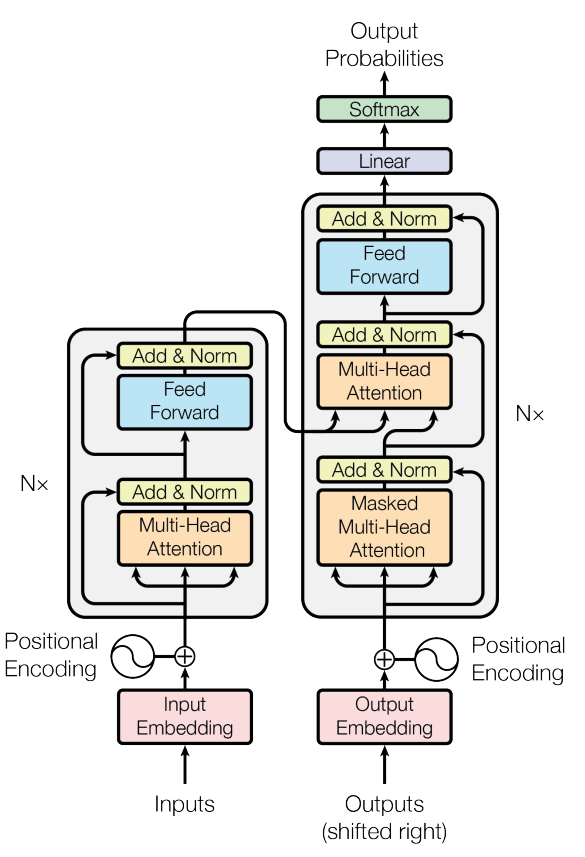
\includegraphics[width=0.4\linewidth]{images/transformer-architecture.png}
    \caption{Transformer architecture ~\cite{vaswani2017attention}}
    \label{fig:transformer_architecture}
\end{figure}
At the core of LLM inference lies the \textbf{context window}, which denotes the maximum number of tokens the model can attend to at any given time. A token is a piece of input, ranging from a subword to even a phrase, depending on the tokenization scheme of the model. For models like LLaMA-2, the context window can be up to 4,096 or 8,192 tokens~\cite{touvron2023llama}. During inference, the model builds an internal representation of this input context, which is used to generate predictions for the next token.

\begin{figure}[h]
    \centering
    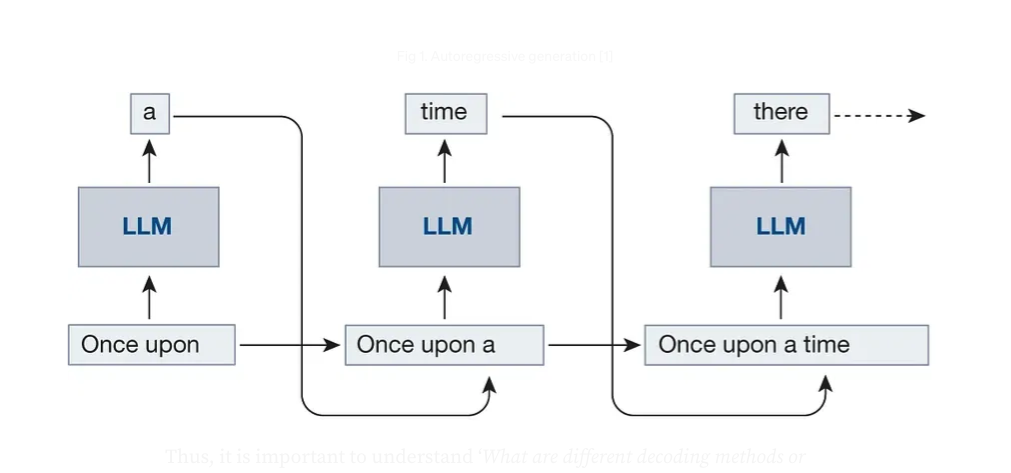
\includegraphics[width=0.6\linewidth]{images/autoregressive-decoding.png}
    \caption{Autoregressive decoding ~\cite{nabi2024all}}
    \label{fig:autoregressive_decoding}
\end{figure}

The \textbf{Key-Value (KV) cache} is a performance optimization central to LLM performance. During autoregressive decoding for text generation, a Large Language Model (LLM) processes the entire input sequence to generate a single output token. This newly generated token is then appended to the sequence, and the model repeats the process iteratively (as seen in Figure ~\ref{fig:autoregressive_decoding}). However, this leads to redundant computation over previously processed tokens at each step. To mitigate this inefficiency, the \textit{key} and \textit{value} vectors computed during the attention mechanism of the transformer can be cached. This \textit{KV caching} technique significantly reduces repeated computation by reusing the stored attention states from prior steps, thereby improving inference speed and memory efficiency. These cached representations allow the model to efficiently attend to all previously generated tokens without recalculating the entire attention graph ~\cite{alammar2018illustrated}. This caching mechanism reduces computational overhead and is especially vital when running LLMs on resource-constrained devices.

Furthermore, the token generation is governed by a sampling algorithm, which yields the output token by sampling on the output probability distribution obtained from the model. Common strategies include greedy sampling, top-$k$ sampling and temperature scaling. A \textbf{token sampler} module is responsible for leveraging these strategies to generate the output token. This can be a resource-hungry step, since this involves processing the probability distribution over the entire vocabulary of the model.

Therefore, the core components required for consistent text generation in an LLM-based system include the model weights, the LLM context (comprising the KV cache and vocabulary), and the token sampler.

Finally, the inference engine managing the model (e.g., llama.cpp, Hugging Face Transformers, or Apple CoreML) orchestrates the context construction, efficient memory handling of the KV cache, and optimized computation for each transformer layer, accounting for quantization if any. These components together define the responsiveness, accuracy, and resource efficiency of the LLM in real-time applications.

%----------------------
\section{LLM Weight Quantization}
\label{sec:LLMWeightQuantization} 
%----------------------
Quantization is a model weight compression technique that reduces the precision of the numbers used for representing model parameters. Typically, reducing the precision from 32-bit floating point to lower-bit integers such as 8-bit, 4-bit, or even 3-bit values. This significantly decreases memory usage and computational requirements, making it possible to run large language models (LLMs) efficiently on edge devices or in real-time environments without sacrificing too much accuracy \cite{jacob2017quantization,hubara2016quantized}.

Within the \texttt{ggml} framework and its application in \texttt{llama.cpp} \cite{llamacpp2023}, various quantization schemes have been introduced to significantly reduce the size and memory footprint of LLM weights. One such scheme is \texttt{Q3\_K\_L}, a 3-bit quantization format specifically designed to balance compression efficiency and model performance \cite{talamdupula2024guide,li2024quantization}. In \texttt{Q3\_K\_L}, weights are grouped in sets of 256 and quantized with shared scaling factors, offset by a zero-point, enabling fine-grained approximation while preserving hardware efficiency. Notably, \texttt{Q3\_K\_L} makes use of 4-bit storage for each quantized value (3 bits for the quantized magnitude and 1 extra bit for improved alignment and bit-packing efficiency), along with 8-bit scales and 6-bit zero-points per group. This layout ensures better alignment with SIMD instructions and allows for faster matrix-vector multiplications, which are critical during transformer inference \cite{pope2022efficiently}. ~\ref{tab:quantization-comparison} shows the comparison between common quantization schemes used in GGML. While this format slightly increases decoding complexity compared to simpler formats like \texttt{Q4\_0}, it provides a favorable tradeoff between model accuracy and size, especially for models deployed in edge or offline settings \cite{ollama2023,llamafile2023}.
Therefore, this project primarily employs model weights quantized using the \texttt{Q3\_K\_L} scheme.

\begin{table}[h]
\centering
\caption{Comparison of Common Quantization Formats in \texttt{ggml}/\texttt{llama.cpp}}
\label{tab:quantization-comparison}
\begin{tabular}{|l|c|c|c|c|}
\hline
\textbf{Format} & \textbf{Bits/Weight} & \textbf{Group Size} & \textbf{Remarks} \\ \hline
Q4\_0     & 4 bits   & 32 weights          & Baseline 4-bit scheme \\ \hline
Q4\_K     & 4 bits   & 64 weights    & Better accuracy than Q4\_0 \\ \hline
Q5\_K     & 5 bits   & 64 weights           & Higher accuracy, more storage \\ \hline
Q8\_0     & 8 bits   & 1 weight                          & No compression, baseline FP8 \\ \hline
\textbf{Q3\_K\_L}  & 3.5 bits avg & 256 weights  & High compression, optimized for SIMD \\ \hline
\end{tabular}
\end{table}


%----------------------
\section{Apple M1 System-on-Chip (SoC)}
\label{sec:AppleM1System-on-Chip} 
%----------------------

The Apple M1 chip, introduced in 2020, is a System-on-Chip (SoC) built on the ARM architecture, which integrates the CPU, GPU, and Neural Processing Unit (NPU) on a single die~\cite{apple2020m1}. This architectural design provides several advantages that are particularly relevant for local inference with large language models (LLMs), particularly for tasks like summarization and question answering.

\begin{figure}[h]
    \centering
    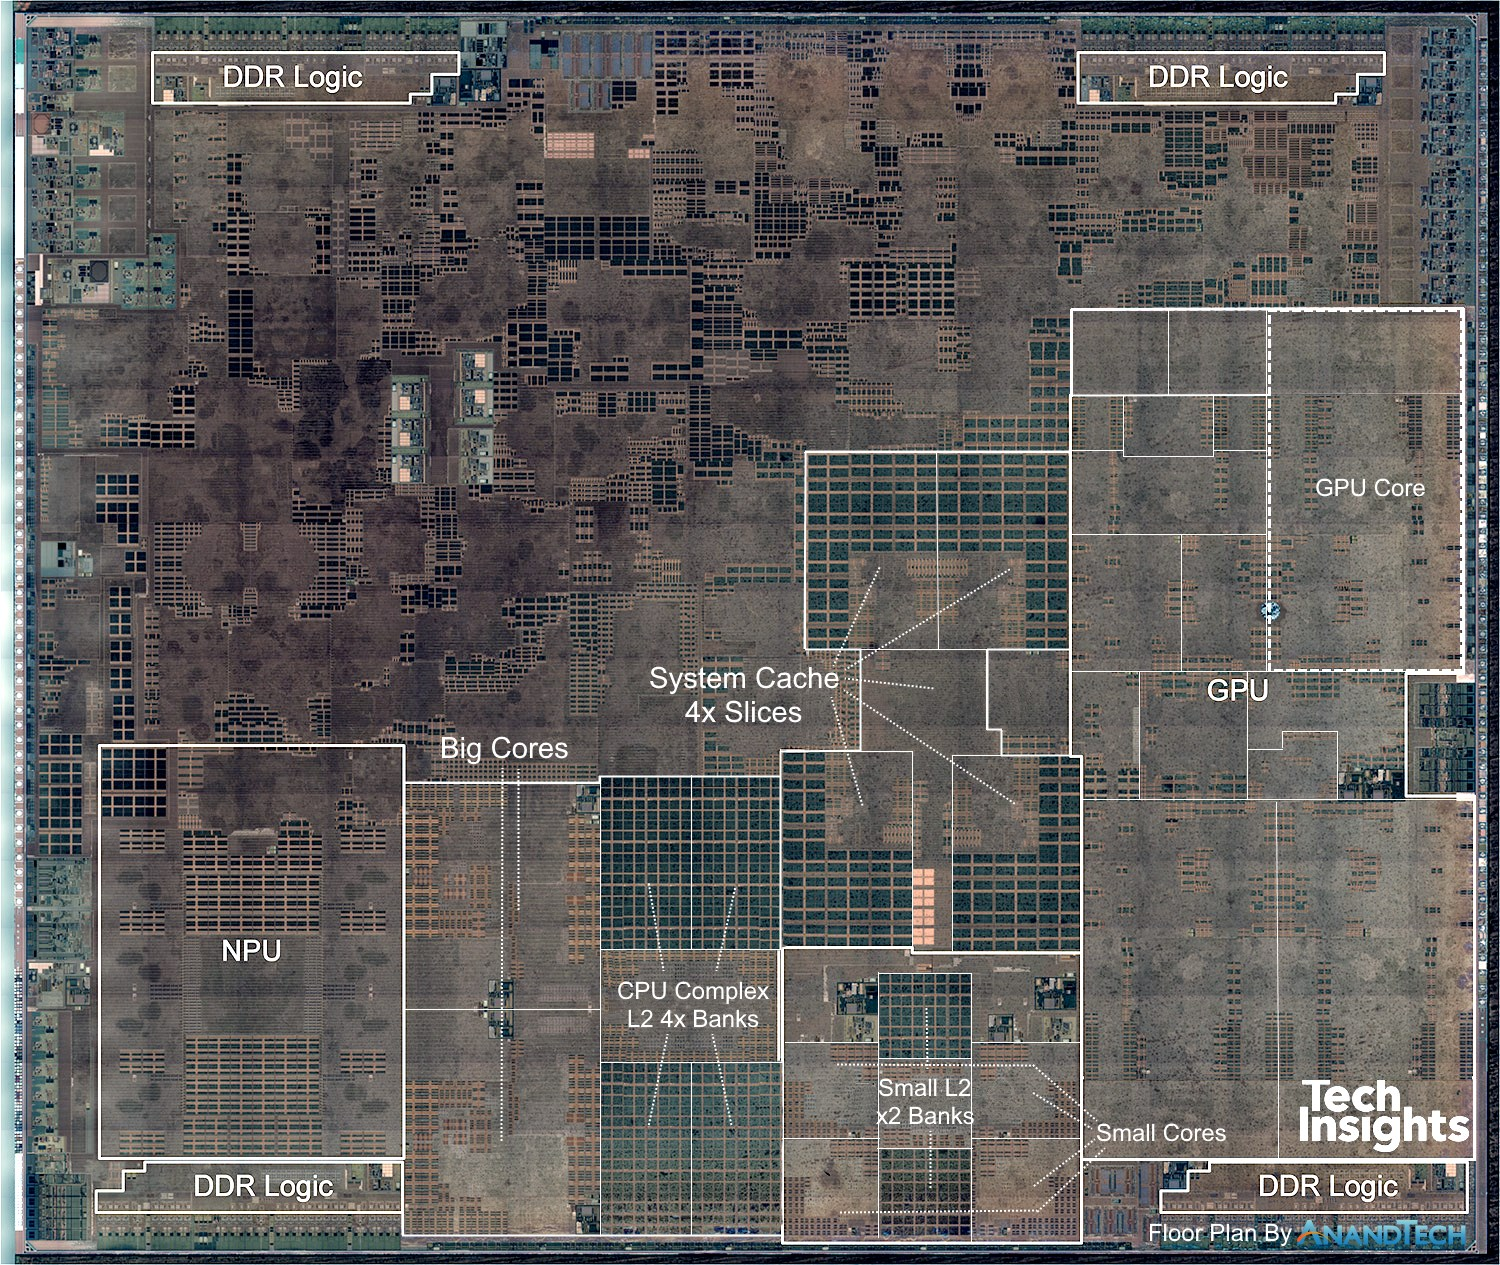
\includegraphics[width=0.8\linewidth]{images/AppleM1SOC.jpeg}
    \caption{ Apple M1 Architecture - (A12 Bionic) Chip floor plan~\cite{hollemans2020apple}}
    \label{fig:autoregressive_decoding}
\end{figure}

\subsubsection*{Unified Memory Architecture}
One of the defining features of the M1 SoC is its Unified Memory Architecture (UMA), which allows the CPU, GPU, and NPU to share the same memory pool \cite{hollemans2020apple}. This eliminates the need for memory copying across processing units and enables zero-copy execution. As a result, applications like retrieval-augmented generation (RAG) benefit from significantly reduced memory overhead and latency. Shared virtual addressing also simplifies software development by allowing seamless access to data structures across different compute units.

\subsubsection*{On-chip Accelerators: GPU and NPU}
The M1 chip includes a built-in GPU with 7--8 cores, capable of delivering up to 5.2 TOPS of performance in INT8 precision \cite{apple2020metal}. It supports general-purpose computation via Metal Shading Language (MSL), analogous to NVIDIA's CUDA, with added features like managed thread indexing and access to 7+ GB of RAM.

The Apple Neural Engine (ANE), or NPU, is an application-specific integrated circuit (ASIC) designed for efficient neural network operations. It offers 11 TOPS of INT8 compute and is exclusively used for machine learning tasks. However, it is only accessible via Apple’s CoreML framework, which supports Swift and Python interfaces. The NPU dynamically collaborates with the CPU, handling SIMD operations like matrix multiplication while delegating sequential logic to the CPU \cite{tinygrad2023apple}.

Unlike the GPU, the NPU is rarely used by general-purpose applications. This makes it a promising candidate for dedicated LLM inference workloads, as its usage is unlikely to interfere with the system's overall responsiveness.

\subsubsection*{Implications for Local LLM Inference}
The M1's integrated architecture is highly beneficial for deploying LLMs locally. Unified memory minimizes data movement, while the GPU and NPU offer parallel computation for matrix-heavy operations common in transformers. Although the NPU cannot be directly accessed via C++ (barring experimental reverse engineering efforts \cite{tinygrad2023apple}), its performance can be leveraged through CoreML model conversion pipelines \cite{apple2024coremlconvert}.

In the context of this project, these capabilities enable a lightweight, resource-efficient desktop application that performs real-time summarization and question answering over a user-provided corpus without relying on cloud resources.



% ============================================================
%
%                   CHAPTER 3: RELATED WORK
%
% =============================================================

\chapter{Related Work}
\label{ch:RelatedWork}
This chapter summarizes current research on Deep Learning (DL) that can be applied in Computational Fluid Dynamics (CFD) to support this study. It describes the current state of DL for CFD and discusses previous work done in this area that differs from this research. Additionally, it presents research that is outside of other areas that can be applied to CFDs.


%----------------------
\section{Potential areas of impact of DL in CFD}
\label{sec:DLinCFD}
%----------------------
The Computational Fluid Dynamics field deals with numerical simulations of fluid flows. Navier-Stokes equations are Partial Differential Equations (PDE) describing fluid flows. Solving those PDEs for chaotic (turbulent) flows requires computationally intensive numerical methods because of the necessary space and time scales. These turbulent flows can be simulated with different accuracy and resource costs. Data-driven modeling methods are revolutionizing scientific discoveries enabled by advances in scientific computing \cite{brunton_data-driven_2022}. Furthermore, Machine Learning and Deep Learning models have the potential to enhance those CFD simulations \cite{vinuesa_enhancing_2022} \cite{brunton_machine_2020}, and recently, there has been an emerging trend of research applications of ML and DL for CFD \cite{vinuesa_emerging_2022}. ML applications in CFD can be categorized into three main areas: Direct Numerical Simulation, Turbulent Modeling, and Reduce Order Models. 

\subsection*{\textbf{Direct Numerical Simulation}}
Direct Numerical Simulations (DNS) provide high accuracy for solving Navier-Stokes equations for fluid flows. Typically, there is a trade-off between the solution's accuracy and feasibility because solving this equation at scale is limited by the computational cost. Some proposed solutions focus on accelerating the numerical simulation by using Deep Learning to approximate parts of the computations involved. For example, \cite{kochkov_machine_2021} developed a method to accurately correct errors caused in low-resolution simulations by learning parameters affected by the coarse grid. They got stable results comparable to high-resolution numerical simulations and reduced the computational cost with a low-resolution discretization grid. Other research \cite{ajuria-illaramendi_towards_2020} \cite{ozbay_poisson_2021} focuses on using DL to solve the Poisson equation for corrections in incompressible fluids. This is done by exploiting data from previous examples to map deviations between uncorrected velocity and the resulting pressure field. 

Those methods only apply ML techniques in part of the solution but still rely on classical numerical methods to calculate the fluid flow. The solution proposed in this research is an end-to-end deep learning model that will apply DL to the entire simulation pipeline with a unified process. This simpler approach has the benefit of eliminating intermediate tasks in the simulation pipeline and thus reducing its complexity.

\subsection*{\textbf{Turbulent Modeling}}
Resolving direct numerical simulations is computationally expensive, so industry CFD applications use Reynolds-Averaged Navier-Stokes (RANS) and Large-Eddy Simulations (LES) methods. Various ML methods used to improve RANS turbulence modeling are explored in \cite{duraisamy_turbulence_2019} to improve its accuracy. Particularly the use of Physics-Informed Neural Networks (PINNs) \cite{wang_physics-guided_2023} \cite{eivazi_physics-informed_2022}. These PINNS models combine the data-driven modeling approach with using physics equations. This combined approach has the advantage of giving the model consistency with known physics laws; however, it makes the solution more complex to implement than a purely data-driven approach. 

In comparison, the model developed in this research is a data-driven approach that can learn from the given data to directly produce predictive results. This approach has the benefit of adapting to the particularities of each use case's data characteristics.


\subsection*{\textbf{Reduce Order Models}}
A useful application of ML in CFD is to develop Reduce Order Models (ROMs) to reduce the data complexity. This can be done because fluid flows contain principal structures that provide essential information about the flow. These ROMs represent the characteristics of the flow in a low-dimension representation that describes the evolution of those principal structures in the fluid, providing a substitute model for faster model predictions. A ROMs technique learns a low-dimensional coordinate system using Proper Orthogonal Decomposition (POD) \cite{taira_modal_2017} \cite{rowley_model_2017}. This technique is related to standard statistics and data-driven modeling techniques for dimensionality reduction: Principal Component Analysis (PCA) and Singular Value Decomposition (SVD) \cite{brunton_data-driven_2022}. Deep Learning can be used to perform those methods in dimensionality reduction by learning the subspace representation from the data \cite{lusch_deep_2018}. Autoencoders are neural networks where the input and output have the same dimensions, but in the middle, there is a bottleneck that reduces the dimensionality of the data. This type of model has two components: the first will take the input and compress it down to a smaller representation with fewer dimensions than the input, and the second one reconstruct the input from the representation. This low-dimensional representation subspace is called latent space and can simplify the original data by compressing it into a smaller representation. Autoencoders can be used to improve the performance of models that rely on classical ROM techniques. Because of the proven advantage of doing dimensionality reduction using DL Autoencoders, this model includes this type of component in its architecture.

%----------------------
\section{Related solutions of DL for CFD}
\label{sec:similarworks}
%----------------------
Recent works have validated the idea of using DL models for CFD modeling using different types of architectures and techniques. Here, we explore research examples that are the most relevant related work to this research, with similar goals but different solutions. It is important to note that although there are some similarities between them and this research, all of them have significant differences, mainly in the dataset used and the proposed architectures.

The use of an extended LSTM network with a Convolutional Neural Network (CNN) and Autoencoders was explored in \cite{mohan_compressed_2019} and \cite{han_new_2019}. Both used an Encoder-Decoder implemented with CNN to compress the data and an LSTM network enhanced with Convolutional filters that use the compressed data to generate the next part of the sequence. \cite{mohan_compressed_2019} develops a data-driven approach for Homogeneous Isotropic Turbulence data in a three-dimensional space. This solution is a sequence-to-sequence model, meaning it gets an initial sequence as input and produces the following sequence as output. The researchers proved that the model achieves good accuracy with long-term stability of the cyclic predictions while being very computationally efficient. \cite{han_new_2019} use a similar model with the same architecture for two-dimensional fluid flows around an obstacle. Their model shows similar results compared with flow fields calculated by a computational fluid dynamic solver. 

A similar method was proposed by \cite{hasegawa_cnn-lstm_2020} to develop ROMs for two-dimensional unsteady flows around a circular cylinder. They also used a CNN for the Autoencoder, with the goal of learning the temporal evolution of the flow in the latent space, they used a much simpler LSTM network. Additionally, they examined the accuracy dependence of this model with different Reynolds numbers (between 20 and 160). Their model was able to reconstruct flows with Reynolds numbers that were not used during the training of the model.

A DL approach to solving Partial Differential Equation systems was proposed in \cite{kakka_sequence_2022}. They developed a sequence-to-sequence model where the Autoencoder was implemented with a Convolutional LSTM. This model was tested with the moving MNIST dataset and the 2-D viscous Burgers equation. The researchers conclude that this model is an excellent network to use when predicting the time series of a dynamical system. Another solution for solving time-dependent PDEs was done in \cite{stevens_finitenet_2020} where they present a machine-learning approach based on a fully convolutional LSTM network to enhance finite-difference and finite-volume methods (FDM/FVM) common to solve PDEs. This method reduced the error by a factor of 2 or 3 compared to baseline algorithms.

A more advanced architecture of DL for CFD was recently proposed by \cite{wang_towards_2024}. The researchers explore the idea of using a combination of $\beta$-variational autoencoders ($\beta$-VAE) \cite{eivazi_towards_2022} to learn a compact representation of the flow velocity and transformers to predict the temporal-dynamics. They use a dataset of a flow around a square cylinder obtained using an open-source numerical simulation with a Reynolds number of 500. They also perform a study to find the optimal values for the $\beta$-VAE, and the effect on model’s performance of hyperparameters such as architecture complexity, regularization $\beta$, and latent vector size. Their model achieves excellent performance, with a 97.8\% of reconstruction accuracy and 96.5\% in temporal-dynamics predictions, demonstrating that this combination has the potential for developing ROMs in complex flows.


%----------------------
\section{Research from other domains}
\label{sec:ResearchOtherDomains}
%----------------------

We also explored other research ideas in the deep learning domain that are not related to CFD applications but can be extrapolated to be applied in this area. These ideas come from video analytics and weather forecasting. We explored how deep learning research in those areas can also be applied to CFD simulations.


\subsection*{\textbf{Video representation and prediction}}
The data for a fluid flow is a sequence of frames representing the state of the fluid at each time; in the same way, a video is a sequence of images in a timeline. Deep learning solutions that can learn features from videos for representation and future prediction have to deal with the same challenges as applications in CFD. In both cases, data has a spatio-temporal structure that requires the model to understand the space and time dimensions to predict future data. In \cite{srivastava_unsupervised_2015}, they use an LSTM neural network to learn representations of video sequences with an autoencoder and then extrapolate the learned video representations into the past and future. They also show that those representations help improve classification accuracy. The architecture is a composite model trained to perform two tasks simultaneously; using the encoded state, the model can predict the next frames as well as input reconstruction. They say that when done separately, the future predictor tends to only store information about the most recent frames, but when the model also has to reconstruct all of the input sequences, it cannot pay attention to just the last frames. This model performance was evaluated using the moving MNIST dataset and 300 hours of YouTube data. It was able to correctly predict the future frames, even when the objects superimpose or bounce while moving.


\subsection*{\textbf{ConvLSTM for precipitation nowcasting}}
Another area where analyzing spatiotemporal data to predict its future evolution is in weather. More specifically, the prediction of future rainfall intensity in a region over a short period of time, also known as precipitation nowcasting. In \cite{shi_convolutional_2015}, they propose a new type of neural network called ConvLSTM by extending the fully connected LSTM by adding convolutional structures. This end-to-end solution is able to outperform LSTM and state-of-the-art methods for the precipitation nowcasting problem. The main reason for this new neural network is that a fully connected LSTM has too much redundancy for spatial data. They mention that this network is not specific for precipitation nowcasting but can also be used for other prediction problems involving spatiotemporal sequence data.



% ============================================================
%
%                   CHAPTER 4: METHODS
%
% =============================================================
\chapter{Methodology}
\label{ch:Methodology}
This chapter outlines the technical methodology adopted in the development of the system, covering both low-level design and software implementation. The approach prioritizes performance, privacy, and modularity, leveraging hardware accelerators where possible and maintaining efficient control over data flow and execution.


%----------------------
%----------------------
\section{Application Modules and Design}
\label{sec:ApplicationDesignModules}
%----------------------

This section provides an overview of the internal architecture and design principles behind the TLDR desktop application. The application is built with the goal of providing a fast, private, and efficient interface for question-answering and summarization tasks over a user-defined corpus of documents. To achieve this, the design incorporates several performance-aware and hardware-conscious modules, especially tailored for Apple’s M1/M2 architecture.

The TLDR system is structured into modular components, each responsible for a specific functionality in the information processing pipeline. These include embedding generation, context retrieval, vector storage, prompt construction, and output generation via a language model. The workflow between these modules is coordinated to support seamless execution, low latency, and high responsiveness, all while maintaining data privacy by running entirely on-device.


%----------------------
\subsection{Overview}
\label{subsec:AppDesignModules-Overview}
%----------------------
The TLDR application follows a modular architecture where different components are responsible for distinct tasks in the RAG (Retrieval-Augmented Generation) pipeline. Figure~\ref{fig:tldr_modules} illustrates the overall design and the control flow between the modules.

\begin{figure}[H]
    \centering
    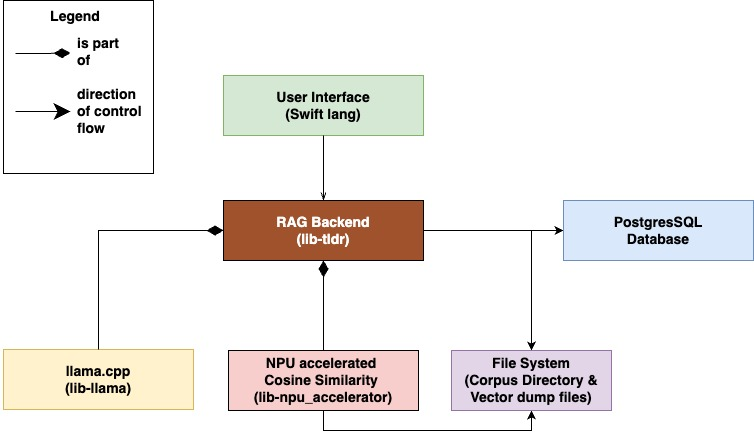
\includegraphics[width=1.0\linewidth]{images/tldr-app-modules.jpg}
    \caption{Modules of TLDR application}
    \label{fig:tldr_modules}
\end{figure}


\begin{itemize}
    \item \textbf{User Interface:} This module provides the graphical frontend for the user. Developed using Swift language for MacOS, it allows users for the users to seamlessly leverage the capabilities of the application. It is responsible for workflows dealing with user experience while delegating all core logic to the backend modules.

    \item \textbf{RAG Backend:} This is the core orchestrator of the application. It manages the full pipeline, including handling user queries, initiating vector search, performing retrieval, and forwarding context to the language model. It communicates with all supporting modules such as the database, NPU based vector search module, llama.cpp and the file system.

    \item \textbf{Database (PostgreSQL):} Stores metadata and document indexing information. It ensures efficient retrieval and persistence of preprocessed documents and vector references. It is plays a crucial role of mapping retrieved vector hashes to their text chunks and document metadata during context retrieval.

    \item \textbf{File System (Corpus Directory and Vector Dump Files):} Contains the document corpus (directory containing source documents) and their corresponding vector dump files. These vector dump are leveraged by the vector search engine using memory-mapped I/O for efficient vector search with low memory overhead.

    \item \textbf{NPU Accelerated Cosine Similarity:} Implements hardware-accelerated cosine similarity by leveraging Apple's Neural Processing Unit (NPU). The backend invokes this module for fast and parallelizable vector cosine similarity computation.

    \item \textbf{llama.cpp:} This module is responsible for language generation i.e LLM inference. It acts as a plugged-in module for the RAG backend and contributes by generating embeddings and chat response during the corresponding stages of the RAG pipeline.
\end{itemize}


%----------------------
\subsection{User Interface}
\label{subsec:AppDesignModules-UI}
%----------------------

The User Interface is in the form of a native MacOS desktop application developed using Swift lang in the Xcode development environment (as depicted in Fig~\ref{fig:tldrGUI}, Fig~\ref{fig:tldrdockicon}). The user interface is designed to be intuitive, lightweight, and self-contained. The application packages all necessary dependencies, including static libraries and LLM weights. enabling fully offline functionality without requiring additional installation or configuration.

The user interface module has the following core purposes:
\begin{itemize}
    \item Provides a clean, chat-style interface where user prompts and LLM responses are displayed as distinct messages to mimic a conversational flow.
    \item Manager all responsibilities regarding user interaction, including persisting user conversation history and any additional user preferences and thereby enable RAG backend to only focus on the RAG functionalities.
    \item \textit{Make a single, self contained portable package that is easy and intuitive to distribute.}
\end{itemize}
\begin{figure}[H]
    \centering
    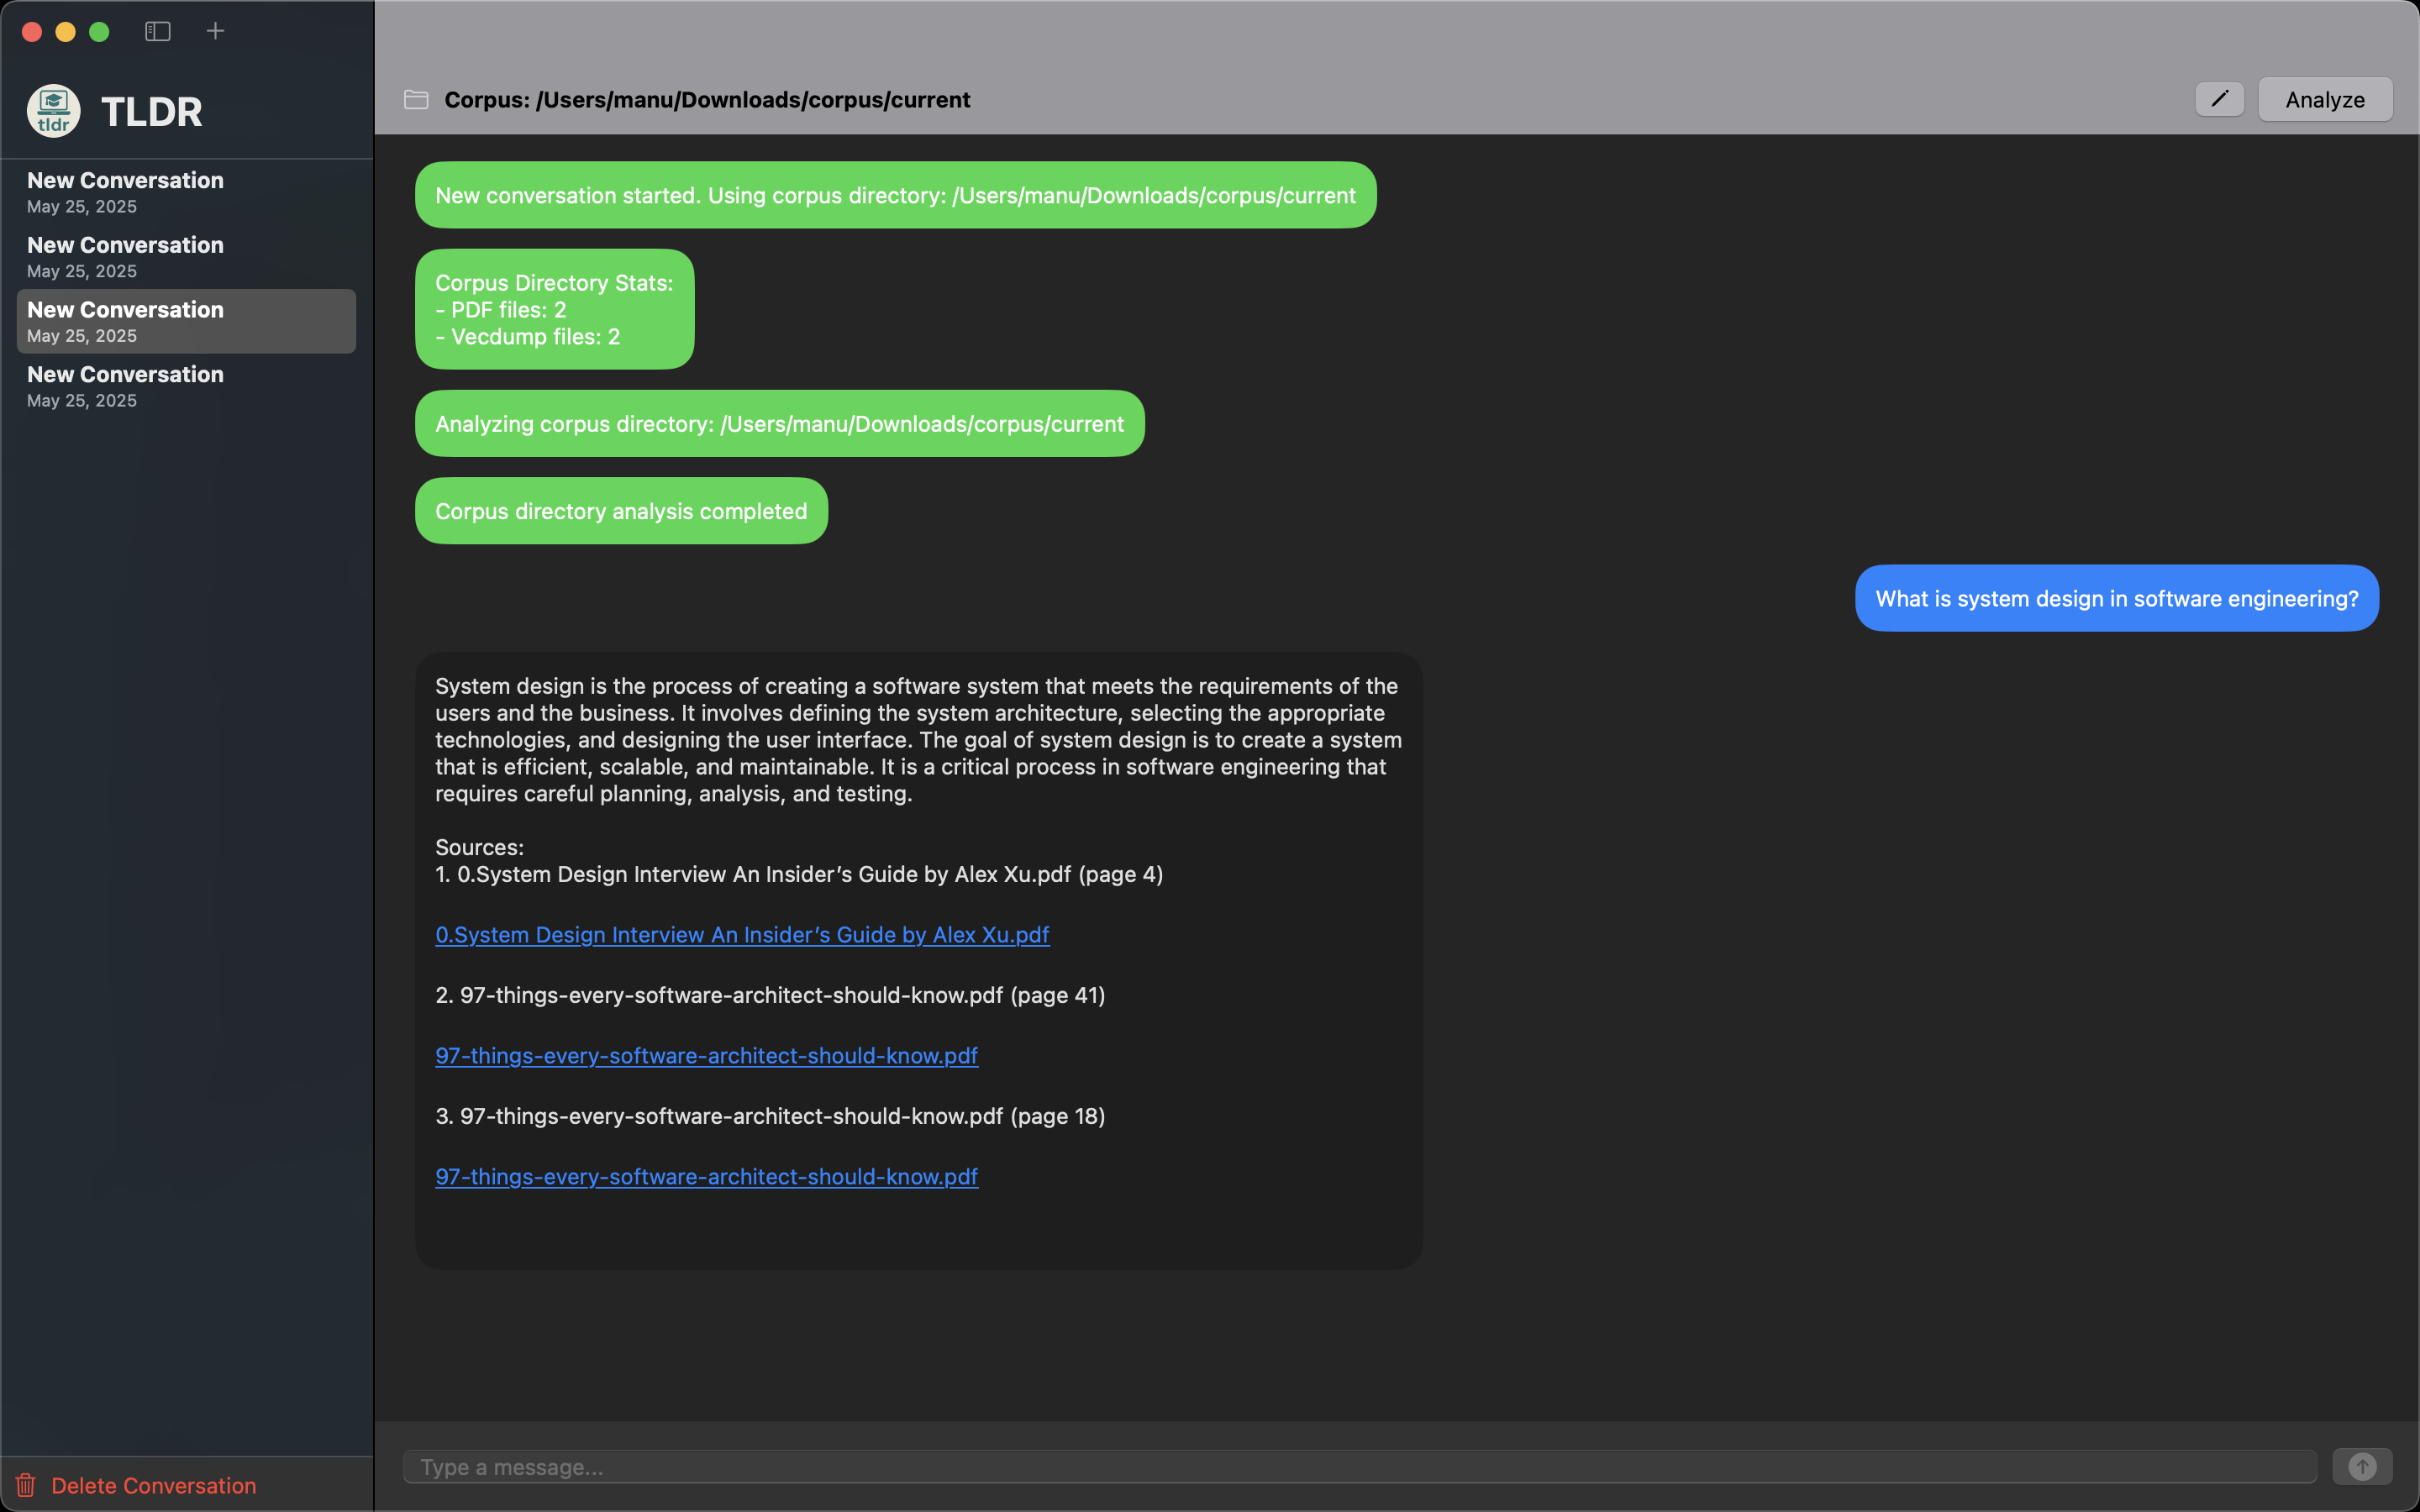
\includegraphics[width=1.0\linewidth]{images/tldr-ui-window.png}
    \caption{Graphical User Interface of TLDR Application}
    \label{fig:tldrGUI}
\end{figure}
\begin{figure}[H]
    \centering
    
\includegraphics[width=0.65\linewidth]{images/tldr-dock-icon.png}
    \caption{TLDR Application Icon as seen in MacOS Dock}
    \label{fig:tldrdockicon}
\end{figure}
%----------------------
\subsubsection{Codebase Organization}
\label{subsubsec:AppDesignModules-UICodebase}
%----------------------

The codebase of the GUI application is illustrated in Figure~\ref{fig:tldrUIFs}. It is organized into several components that serve both core functionality and supporting roles within the application. 
\begin{figure}[H]
    \centering
    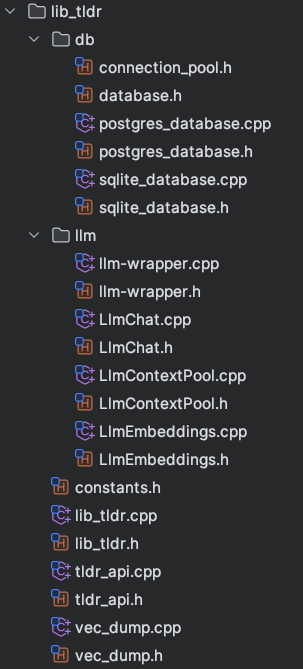
\includegraphics[width=0.5\linewidth]{images/ui-proj-fs.png}
    \caption{UI Project File system}
    \label{fig:tldrUIFs}
\end{figure}
\begin{enumerate}[label=\Alph*.]
    \item Overall Structure:
    \begin{enumerate}[label=\alph*.]
        \item \texttt{tldr}: The Swift language codebase that creates the user interface.
        \item \texttt{TldrAPI}: C++ module with bindings for Swift UI. It serves as a bridge between the Swift UI and the C++ static library of the RAG Backend.
    \item \texttt{artefacts}: Quantized LLM weights and coreml packages, i.e:
    \begin{itemize}
        \item \texttt{Llama-3.2-1B-Instruct-Q3\_K\_L} model for chat
        \item \texttt{all-MiniLM-L6-v2-Q8\_0} model for generating embeddings
        \item \texttt{CosineSimilarityBatched} coreml package for cosine similarity on NPU
    \end{itemize}
    \end{enumerate}

    \item UI Architecture (MVVM):
    \begin{enumerate}[label=\alph*.]
        \item \texttt{tldrApp}: The main SwiftUI entry point where the application lifecycle begins.
        \item Models: Includes \texttt{ConversationData}, \texttt{Message}, and \texttt{RagResultSw} to represent the chat state and RAG outputs. These modules leverage \textit{UserDefaults} a built-in key-value persistance mechanism provided by Apple's Foundation framework to efficiently store and retrieve their information.
        \item Views: Comprises SwiftUI components like \texttt{ChatView} and \texttt{ContentView} to render the main interface.
        \item ViewModels: Contains \texttt{ChatViewModel}, which handles user interaction and backend coordination.
        \item Preview Content: Includes \texttt{Preview Assets} for SwiftUI previews to support development and layout testing.
        \item Assets: Stores static resources such as icons and other UI elements.
    \end{enumerate}
\end{enumerate}
This organization promotes maintainability and allows for a clear separation of concerns between UI presentation, interaction logic, and backend communication.
%----------------------
\subsection{RAG Backend}
\label{subsec:AppDesignModules-RAG Backend}
%----------------------
\begin{figure}[htbp]
  \centering
  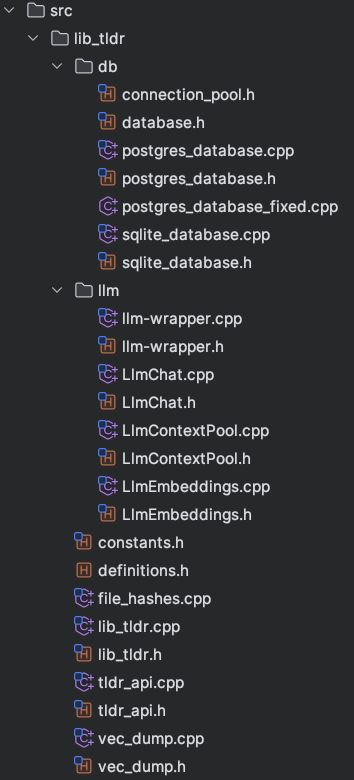
\includegraphics[width=0.5\linewidth]{images/lib_tldr_fs.png}
  \caption{RAG Backend(lib\_tldr) codebase}
  \label{fig:libTldrCodebase}
\end{figure}

The RAG backend is implemented as a C++ static library named \texttt{lib\_tldr}. It serves as the backbone for all core functionalities of the project. This module encapsulates the complete RAG pipeline logic and integrates essential components such as the large language model for text and embedding generation, the vector dump generator and reader, database and file system handlers for storage, and the cosine similarity-based vector retriever (as seen in Fig~\ref{fig:libTldrCodebase}).

The architecture emphasizes modularity and resource efficiency, enabling plug-and-play replacement or extension of components. It adheres to the SOLID principles of object-oriented programming, promoting adaptability, maintainability, and scalability.



Following are the logical sub-modules of RAG Backend:
\begin{enumerate}[label=\Alph*.]
\item{Language Model Interface:}

The system utilizes \texttt{llama.cpp} as the backend for both text generation and embedding extraction. The following components facilitate this integration:

\begin{enumerate}
    \item \texttt{LlmChat.cpp \&.h}: Manage the logic to take user input and retrieved context and generate a response from the chat LLM. 
    \item \texttt{LlmEmbeddings.cpp \&.h}: These modules extract dense vector representations (embeddings) from document chunks, which are subsequently used for semantic similarity search and retrieval.
    \item \texttt{LlmContextPool.cpp \&.h}: These components manage the lifecycle of LLM context objects, which encapsulate the model state necessary for efficient inference. Since LLMs typically require a context to maintain internal buffers, tokenizer state, and memory allocations, it is computationally expensive to initialize a new context for every query or embedding operation. By pooling and reusing contexts across multiple operations, the system significantly reduces initialization overhead and ensures smoother, low-latency performance during both chat and embedding workflows.
    \item \texttt{Llm-Wrappers.cpp \&.h}: Takes care of initializing and cleaning up resources related to the LLMs. It initializes common ggml backend for Apple metal and setting up LLM context pools and initialize Chat and Embedding LLMs by loading their weights into memory.
\end{enumerate}

\item{Database Interaction:}
All persistent storage is handled via the PostgreSQL backend, though an optional SQLite backend is also implemented (but not currently utilized). The database interaction is managed within the \texttt{db} submodule, which includes the following:

\begin{enumerate}[label=\alph*.]
\item \texttt{database.h}\: Defines an abstract class that enforces a uniform interface for any underlying database implementation. This design allows the RAG codebase to remain unchanged when switching between different database technologies.
    \item \texttt{postgres\_database.cpp \&.h}: These files handle database initialization, schema definition, and CRUD operations related to documents and embeddings in PostgreSQL Database.
    \item \texttt{connection\_pool.h}: Provides a lightweight connection pooling mechanism to manage multiple concurrent database sessions efficiently. This is especially beneficial during large-scale embedding operations where multiple inserts are performed rapidly. It is efficient to store readily available connections and re-use them instead of creating a new connection for every db interaction.
\end{enumerate}

The PostgreSQL schema stores both high-level document metadata (e.g., title, author, page count) and low-level embedding-related information (e.g., text chunk, hash, embedding vector, page number, and timestamps).

\item{Embeddings Vector Storage and Retrieval\:}

\texttt{vec\_dump.cpp \&.h}  are responsible for managing the serialized storage of raw vector data ("vecdumps"). These are binary representations of embedding vectors that can be rapidly accessed and processed.

Additionally, the system incorporates a hardware-accelerated module referred to as the \texttt{npu-accelerator}, which leverages macOS’s Neural Engine to perform cosine similarity search over large sets of embeddings. This offloads compute-intensive operations from the CPU, enabling real-time retrieval performance on resource-constrained devices.

\item{Core Workflow:}
The \texttt{lib\_tldr.cpp \&.h} contains the core logic that glues the entire system together, such as:
\begin{itemize}
    \item Initializing the LLMs and the Database tables (when necessary)
    \item Creating DB connection pool and LLM context pool
    \item Checking for changes in the corpus directory and embedding new documents
    \item Performing Retrieval Augmented Generation
    \item Cleaning up and releasing acquired resources
\end{itemize}


\item{RAG Backend API:}
While the backend contains numerous functions and data structures for internal logic, a clean and minimalistic API (Application Programming Interface) is exposed. This allows its client modules (such as the UI module) to leverage its capabilities without being closely coupled with the internal mechanisms of the library.

The \texttt{tldr\_api.cpp \&.h} files expose a clean, C-style API interface for the user-facing application layer on top of the functions present in \texttt{lib\_tldr.cpp \&.h}. 

\end{enumerate}

 %----------------------
\subsection{Database (PostgreSQL)}
\label{subsec:AppDesignModules-DatabasePSQL}
%----------------------
The application uses PostgreSQL as its persistent storage backend to manage and retrieve embedding data required during the Retrieval-Augmented Generation (RAG) process. The database stores preprocessed document chunks, their vector embeddings, associated metadata, and file-level information.

PostgreSQL was chosen over lighter-weight alternatives like SQLite due to its superior concurrency handling. Specifically, SQLite’s single-writer limitation presented a bottleneck in the multi-threaded embedding pipeline, where concurrent writes to the embedding store are common. PostgreSQL’s support for multiple concurrent writers allows the embedding process to scale efficiently without serialization delays.

\subsubsection{Table: documents}
This table stores metadata for each unique input file in the corpus. It ensures file-level uniqueness through the \texttt{file\_hash} field and includes fields such as file name, author, subject, page count, and timestamps. It acts as a parent entity in a one-to-many relationship with the \texttt{embeddings} table (refer to table definition in Fig~\ref{fig:psqlDocumentTableDesc}). 

\begin{figure}[H]
    \centering
    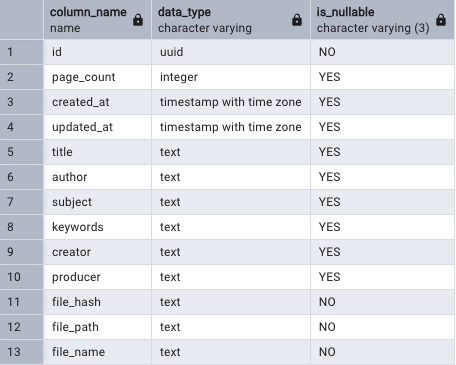
\includegraphics[width=0.7\linewidth]{images/dbtable-documents.png}
    \caption{Documents table description}
    \label{fig:psqlDocumentTableDesc}
\end{figure}


\subsubsection{Table: embeddings}

This table stores the chunk-level data required for semantic search. Each row contains a reference to a document, the original text chunk, its embedding vector, and an embedding hash. During query time, the vector search module returns the top-$K$ most similar vectors based on cosine similarity. The corresponding text chunks are then retrieved from this table using the hash and document ID to form the LLM context (refer to table definition in Fig~\ref{fig:psqlEmbeddingsTable}).

\begin{figure}[H]
    \centering
    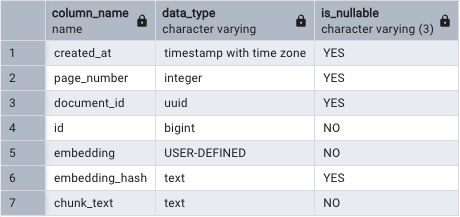
\includegraphics[width=0.7\linewidth]{images/dbtable-embeddings.png}
    \caption{Embeddings table description}
    \label{fig:psqlEmbeddingsTable}
\end{figure}
%----------------------
\subsection{File System: Corpus Directory and Vectordump Files}
\label{subsec:AppDesignModules-FSandVectordump_files}
%----------------------
Vector dump files are binary data structures designed for efficient storage of document embeddings. For each input document, a corresponding vector dump file is created. Each such file contains embedding vectors generated from text chunks along with their corresponding MD5 hashes. This format enables fast similarity search and content verification in document retrieval systems.

%----------------------
\subsubsection{Corpus Directory}
\label{subsec:AppDesignModules-CorpusDir}
%----------------------
The corpus directory serves as the source of truth for the RAG pipeline. It contains the raw documents—primarily PDF files—that are parsed, chunked, and processed by the language model to construct the knowledge base used for information retrieval. 

This project recursively scans the specified corpus directory, identifies all PDF files, computes their corresponding embeddings, and stores them in \texttt{.vecdump} files.
%----------------------
\subsubsection{Vectordump Files}
\label{subsec:AppDesignModules-Vectordump_FileStructure}
%----------------------
Vector dump files are obtained as a result of the embedding process. After a document is split into chunks, each chunk is processed by the LLM and yields embeddings. Embeddings are higher dimensional representations of the input text, as interpreted by the LLM. 
These embeddings are then stored in a dedicated subdirectory named \textit{\_vecdump}, located within the corpus directory itself. The \textit{\_vecdump} folder houses binary \texttt{.vecdump} files that are later used during the similarity search phase to efficiently retrieve semantically relevant chunks.

The vector dump file follows a sequential binary layout consisting of three main components: a metadata header, followed by embedding data, and finally hash data (as illustrated in Fig~\ref{fig:vectordumpfilestructure}. This structure allows for efficient random access to embeddings while maintaining data integrity through hash verification. Hash is also further used for fetching the corresponding text chunk after similar vectors are obtained for a query.

   \begin{figure}[h]
    \centering
    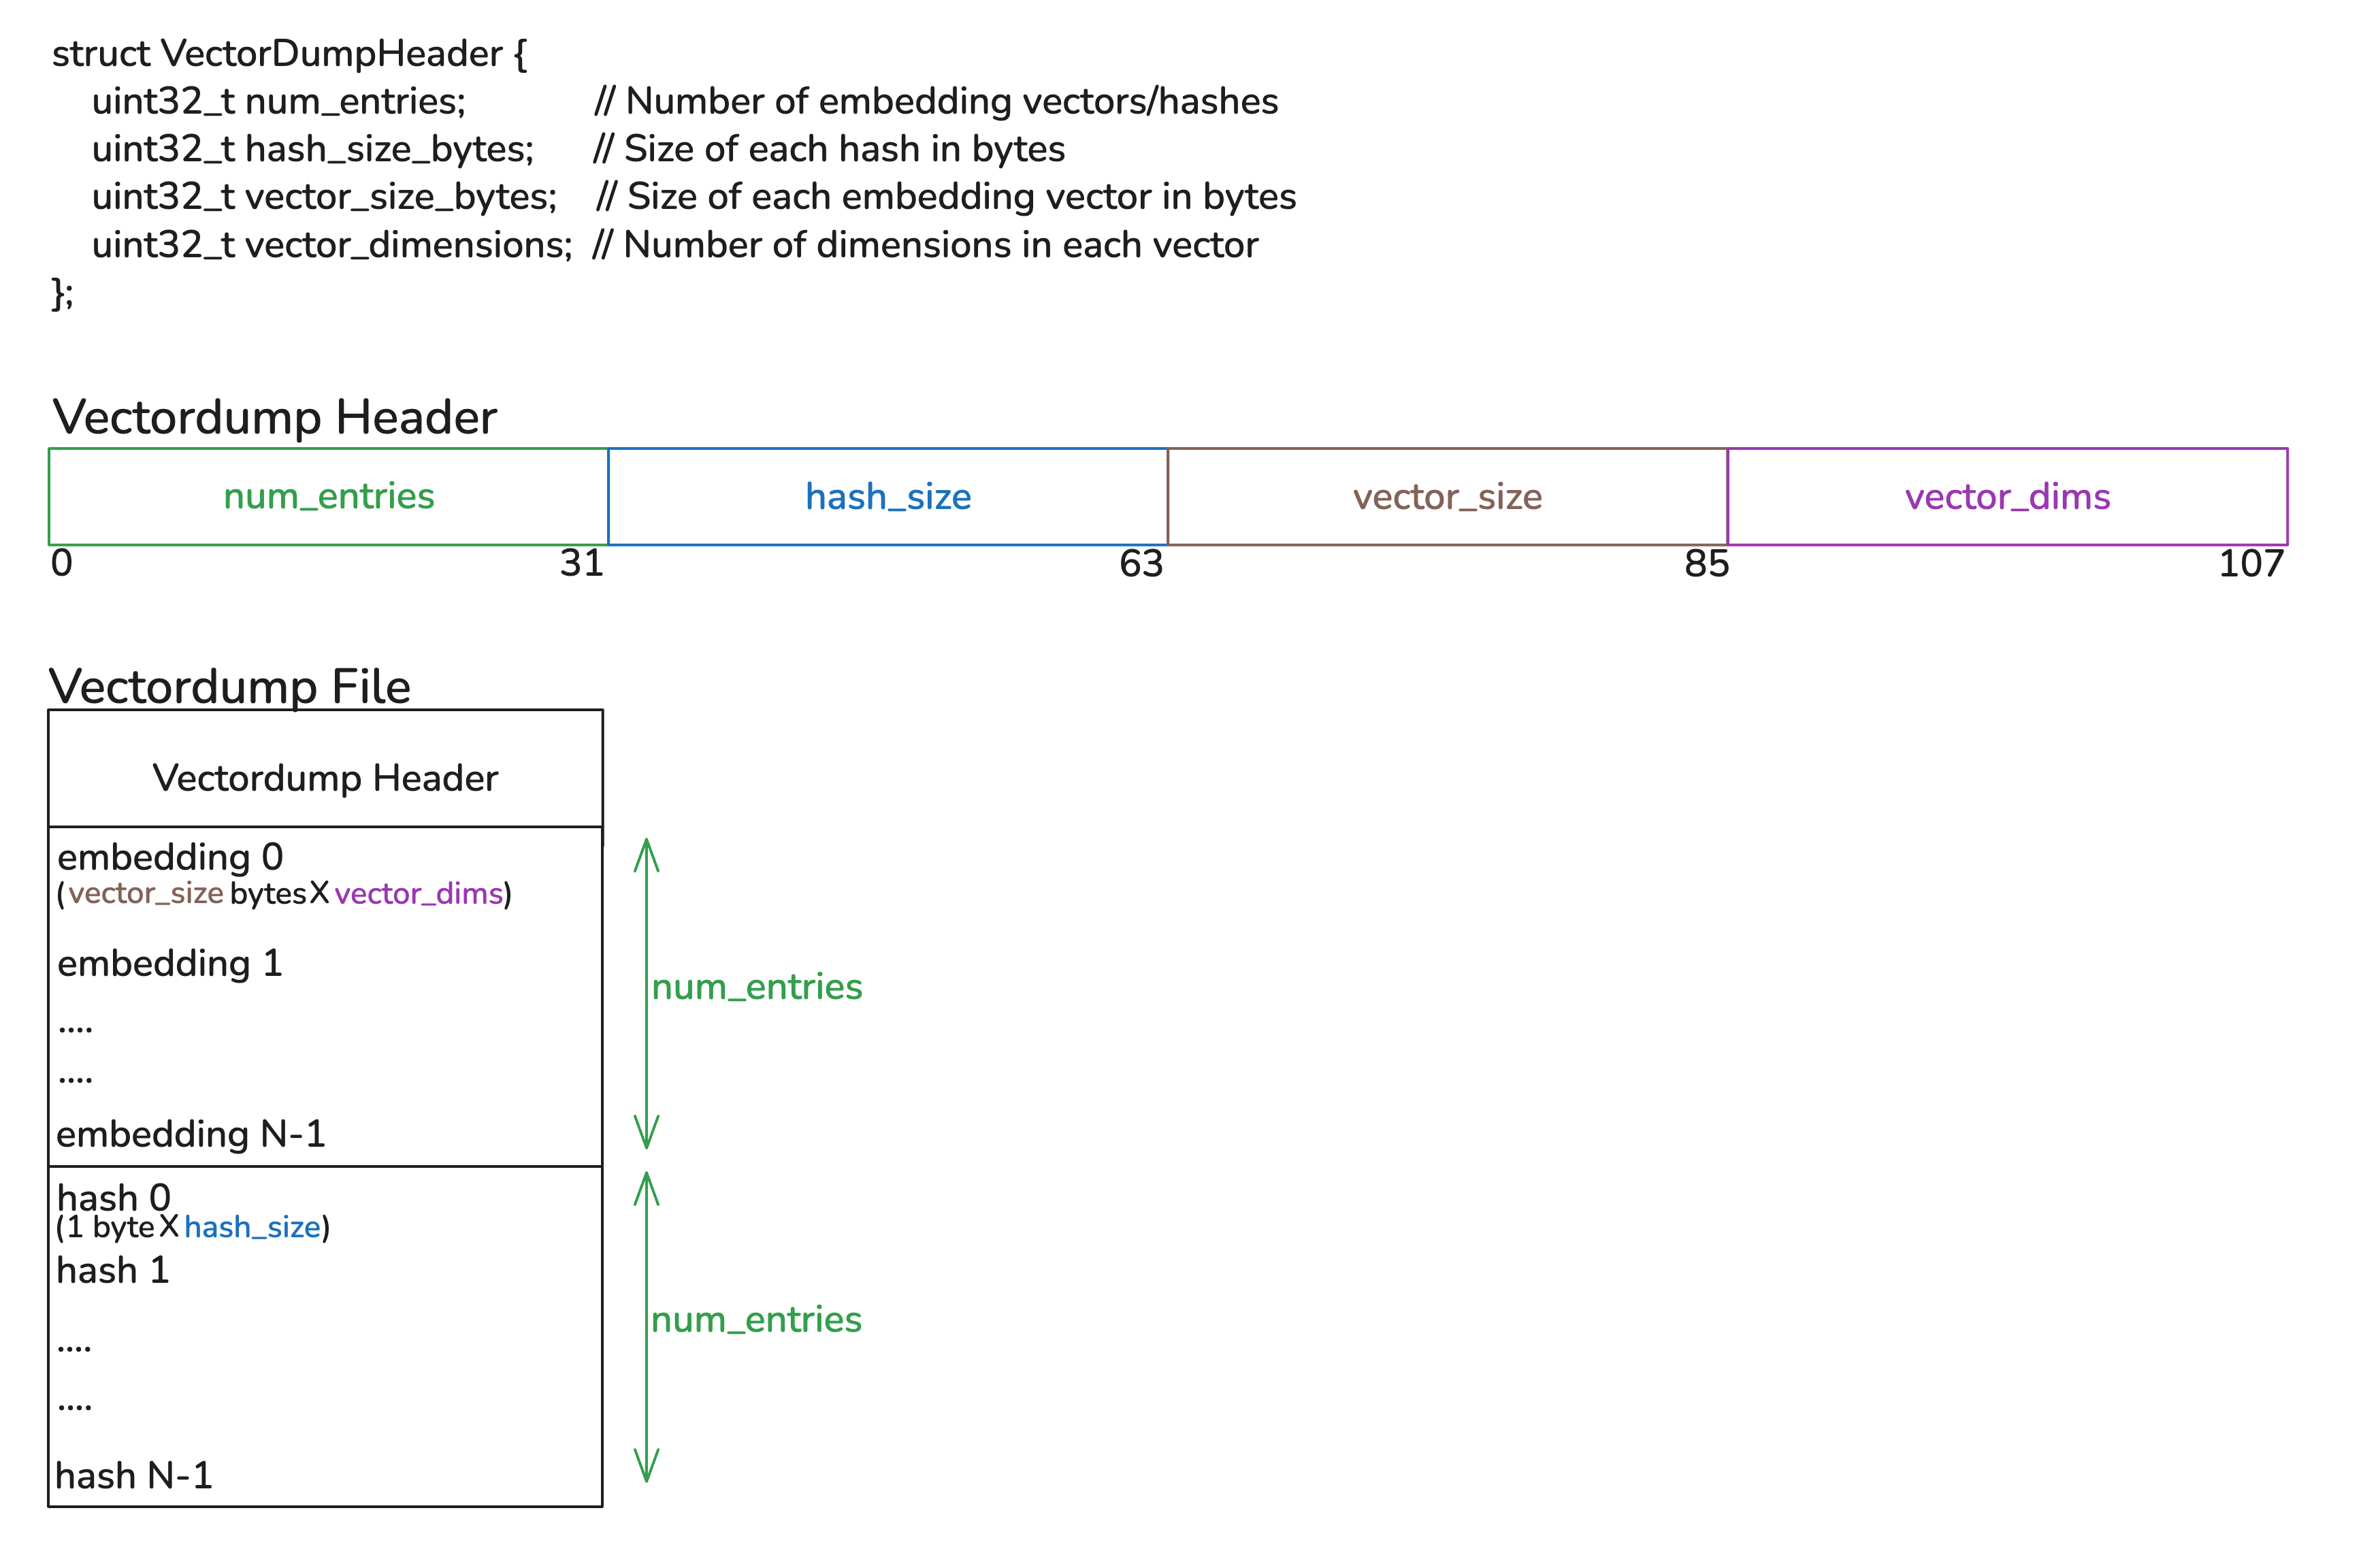
\includegraphics[width=0.9\linewidth]{images/VectorDumpFiles.png}
    \caption{Vector dump file structure}
    \label{fig:vectordumpfilestructure}
\end{figure}

%----------------------
\subsubsection{Vectordump Header}
\label{subsec:AppDesignModules-Vectordump_Header}
%----------------------
In order to process the vector dump file, the header is first read and the necessary information is obtained regarding the data layout in the file. The information is arranged in the layout as illustrated in Figure~\ref{fig:vectordumpfilestructure}. The elements are as follows:
\begin{itemize}
    \item \texttt{num\_entries} - Total number of embedding/hash pairs stored in the file
    \item \texttt{hash\_size\_bytes} - Size of each MD5 hash in bytes (always 16 for standard MD5)
    \item \texttt{vector\_size\_bytes} - Total byte size of each embedding vector
    \item \texttt{vector\_dimensions} - Number of floating-point dimensions per embedding vector
\end{itemize}

The header is read by simply pointing a pointer of type $struct VectorDumpHeader$ to the memory location to which the file is loaded. This helps obtain the necessary information required to access the data sections of the file.

%----------------------
\subsubsection{Data Sections}
\label{subsec:Vectordump_DataSections}
%----------------------
Once the header section is loaded, the data obtained is then used for calculating the memory locations of the embedding and hash arrays.
Pointers are used to access these locations to simulate the structure of an array on top of raw binary data read into the memory. This approach is simple and efficient and prevents needless memory allocations and data copies.

\textbf{Embeddings:} Contains $N$ consecutive embedding vectors, where $N$ = \texttt{num\_entries}. Each vector occupies \texttt{vector\_size\_bytes} and represents a \texttt{vector\_dimensions}-dimensional embedding, stored as 32-bit floating point values. In the current case, we use a 384-dimensional vector embedding.

\textbf{Hashes:} Contains $N$ consecutive MD5 hash values, each exactly 16 bytes. However, the smallest unit of storage is of $uint64_t$ type, i.e., units of 2 bytes. Hence, a 16 byte MD5 hash would have a hash size of 8. The hash at index $i$ corresponds to the MD5 digest of the original text chunk used to generate \texttt{embedding[i]}.


%----------------------
\subsubsection{Data Relationship}
\label{subsec:Vectordump_DataRelationship}
%----------------------

The file maintains strict positional correspondence: for any index $i \in [0, N-1]$, \texttt{embedding[i]} and \texttt{hash[i]} represent the same document chunk. This one-to-one mapping enables efficient lookup operations and integrity verification during retrieval.

The data is used as follows:
\begin{enumerate}[label=\arabic*.]
\item Load the first half of the file in memory using \textbf{mmap} and perform cosine similarity search.
    \item Obtain index of the top $K$ relevant vectors from Cosine similarity module.
    \item Fetch the hash values at the obtained indices.
    \item Query the database for text chunks associated with the hash values.
\end{enumerate}
    
This design allows for prioritized access to necessary data and its direct usage for cosine similarity search with no further processing or data manipulations, allowing for an efficient search through the entire corpus.

%----------------------
\subsection{NPU Accelerated Cosine Similarity}
\label{subsec:AppDesignModules-NpuCosineSim}
%----------------------
The NPU accelerator module (lib-npu\_accelerator) is a specialized component of the TLDR MacOS desktop application that leverages Apple's Neural Processing Unit to perform hardware-accelerated cosine similarity computations as part of the RAG pipeline.
The module construction and usage is a multi-step process involving multiple components. The codebase structure is depicted in Fig~\ref{fig:libnpucodebase} and the workflow in Fig~\ref{fig:libnpuworkflow}.

\subsubsection{Codebase structure}
The codebase for the npu module as seen in Fig~\ref{fig:libnpucodebase} has the following components:
\begin{figure}[h]
    \centering
    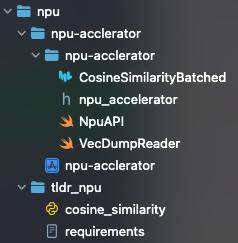
\includegraphics[width=0.4\linewidth]{images/npu-fs.png}
    \caption{lib-npu\_accelerator codebase}
    \label{fig:libnpucodebase}
\end{figure}
\begin{itemize}
    \item \textbf{PyTorch module (\texttt{tldr\_npu}):} Contains PyTorch code to perform batched cosine similarity. This module is used to generate a CoreML model package, which is later utilized by the NPU accelerator for high-performance similarity computation.
    \item \textbf{Swift module (\texttt{npu-accelerator}):} Implements the logic in Swift to read vector dump files and leverage the CoreML cosine similarity model to perform efficient vector similarity search using the Apple Neural Engine (ANE).
\end{itemize}

\subsubsection{Processing Workflow}

\begin{figure}[h]
    \centering
    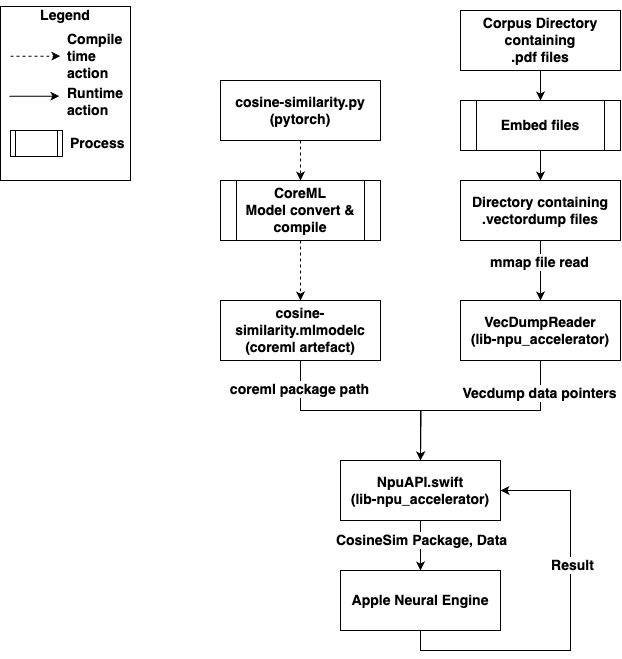
\includegraphics[width=0.7\linewidth]{images/npu-accelerator-module-worklfow.jpg}
    \caption{NPU accelerator module workflow}
    \label{fig:libnpuworkflow}
\end{figure}
The NPU accelerator workflow could be visualized as  dual-pipeline workflow as illustrated in Fig~\ref{fig:libnpuworkflow}. 

\textbf{Phase I - Prepare the components}:
The left pipeline begins with a PyTorch-based cosine-similarity.py implementation that serves as the foundation for similarity computations. This PyTorch model undergoes a CoreML model conversion and compilation process, transforming the original implementation into an optimized CoreML artifact specifically designed for Apple's Neural Engine execution. The compilation step produces the \textit{cosine-similarity.mlmodelc} package, which contains the optimized model ready for hardware acceleration.

The right pipeline operates in parallel, handling document processing and vector storage. Although this portion of the pipeline is  executed by the RAG Backend and is not directly part of the NPU module, it still is a logical component of the NPU module workflow as depicted in Fig~\ref{fig:libnpuworkflow}.

\textbf{Phase II - Perform vector search}:
This phase is triggered at runtime when a user submits a query and the RAG pipeline is activated. The workflow converges at \texttt{NpuAPI.swift}, a Swift-based interface that integrates the CoreML similarity model and the document embeddings obtained via the \texttt{VecDumpReader}.

The \texttt{VecDumpReader} accesses vector dump files using memory-mapped I/O (\texttt{mmap}), exposing the data as raw pointers without intermediate copies. These pointers are passed directly to the \texttt{CosineSimilarityBatched} module, which performs batched cosine similarity computations using Apple's Neural Engine (ANE).

\texttt{NpuAPI} orchestrates this process by coordinating the CoreML model execution and the memory-resident embeddings, enabling efficient hardware-accelerated similarity search. The output consists of similarity scores and embedding hash values, which are used by the RAG system to retrieve the most relevant document chunks for generating a contextually informed response. Furthermore, \texttt{NpuAPI} also serves as a bridge to the C++ layer, exposing these capabilities to the RAG backend for use during the retrieval phase of the RAG pipeline.

Although cosine similarity involves a full scan of the embedded corpus for each query, the system architecture mitigates performance concerns through the following mechanisms:

\begin{itemize}
    \item \textbf{Shared memory-mapped files:} When multiple threads handle different user requests, redundant file reads are avoided because the \texttt{mmap} mechanism loads the file into memory only once.
    
    \item \textbf{Zero-copy access:} Since the data is accessed directly from memory without duplication, there is no overhead for repeated reads. Additionally, the operating system can page the data out to swap memory and page it back in when needed, optimizing memory usage.
    
    \item \textbf{Unified memory architecture:} The Apple M1/M2 SoC’s unified memory architecture enables seamless access between CPU, GPU and NPU, eliminating the need for further data transfers during vector similarity computations.
\end{itemize}

%----------------------
\subsection{llama.cpp}
\label{subsec:AppDesignModules-LLaMaCpp}
%----------------------

The project integrates a customized fork of \texttt{llama.cpp}—a lightweight C++ inference engine for LLaMA and related transformer models—to serve as the core engine for both text generation and embedding extraction. The fork is hosted at \url{https://github.com/manuhg/llama.cpp}, and includes minor modifications that streamline the build process for macOS targets. Specifically, the build scripts were stripped down to produce a static library using the \texttt{ggml} Metal backend, optimized for Apple Silicon devices.  The result is a single, portable C++ static library named \texttt{libllama.a} which is then statically linked with the RAG backend (\texttt{lib-tldr.a}).

The core functionalities such as tokenization, decoding, and sampling are accessed through the public APIs exposed in \texttt{llama.h} and \texttt{ggml.h}. Two primary components—\texttt{LLmChat} and \texttt{LLmEmbedding}—are built around workflows inspired by \texttt{simple.cpp}~\cite{llama_simple} \texttt{server.cpp}~\cite{llama_server} and \texttt{embedding.cpp}~\cite{llama_embedding} from the upstream \texttt{llama.cpp}~\cite{llamacpp} project. 

Further, to improve the performance, \texttt{OpenMP} support was added for parallelizing the tokenization and batch decoding steps. This optimization ensures efficient utilization of CPU cores, resulting in faster preprocessing and inference, particularly during multi-threaded interactions.

The \texttt{llama.cpp} is hence directly integrated into the RAG backend at compile time. This enables the application to perform in-memory LLM inference by directly invoking components of \texttt{llama.cpp}, without relying on any external dependencies or background processes for this core functionality.
%----------------------
%----------------------
\section{Application Workflow}
\label{sec:AppWorkflow}
%----------------------

%----------------------
\subsection{Workflow Overview}
\label{subsec:AppDesignWorkflow-Overview}
%----------------------

\begin{figure}[H]
    \centering
    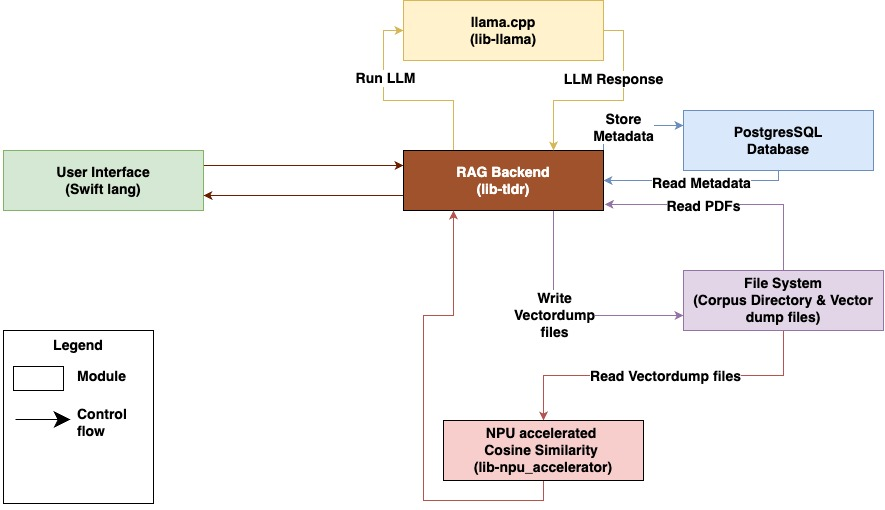
\includegraphics[width=1.0\linewidth]{images/tldr-app-module-interactions.jpg}
    \caption{TLDR application module interactions}
    \label{fig:tldrmodulesinteraction}
\end{figure}

Figure~\ref{fig:tldrmodulesinteraction} illustrates the high-level architecture of the TLDR application, highlighting its modular design and control flow between components.

At the center is the \textbf{RAG Backend} (\texttt{lib-tldr}), which serves as the core orchestrator. It interfaces with several specialized modules to perform retrieval-augmented generation.

\begin{itemize}
    \item The \textbf{User Interface}, interacts with the RAG backend to initiate queries and display responses to the user.
    
    \item \textbf{llama.cpp} (\texttt{lib-llama}) is linked as a static library and provides language model functionality. The backend calls it for both text generation and embedding, receiving outputs directly in memory.
    
    \item \textbf{PostgreSQL Database} is used to store and retrieve document metadata and precomputed embeddings. The RAG backend communicates with it to persist and query structured data including document metadata and text chunks for embeddings.
    
    \item The \textbf{File System} acts as the persistent store for documents and vector dumps. The backend reads PDF files for embedding and writes embedding outputs into binary vector dump files.
    
    \item \textbf{NPU-Accelerated Cosine Similarity} (\texttt{lib-npu\_accelerator}) reads the vector dump files through memory-mapped I/O and executes similarity search using a CoreML model on Apple's Neural Engine (ANE).
\end{itemize}

This modular architecture allows each component to focus on a specific responsibility while maintaining efficient communication with the core backend. All dependencies are statically compiled or locally integrated, ensuring portability and performance.


%----------------------
\subsection{RAG Pipeline Workflow}
\label{subsec:RAGWorkflow}
%----------------------
The workflow of the modules of the system and the RAG pipeline can be divided into 3 logical phases. 
\begin{itemize}
    \item System Initialization: Initializes the resources required by the system.
    \item Embedding Phase: Generate embeddings for documents in the source corpus.
    \item Retrieval and Generation Phase: Leverage embedded documents to retrieve information relevant to a query made by the user and generate a response using the LLM.
\end{itemize}
The following sections show a detailed breakdown of these phases.

%----------------------
\subsubsection{System Initialization}
\label{subsec:AppDesignWorkflow-SystemInitialization}
%----------------------

\begin{figure}[H]
    \centering
    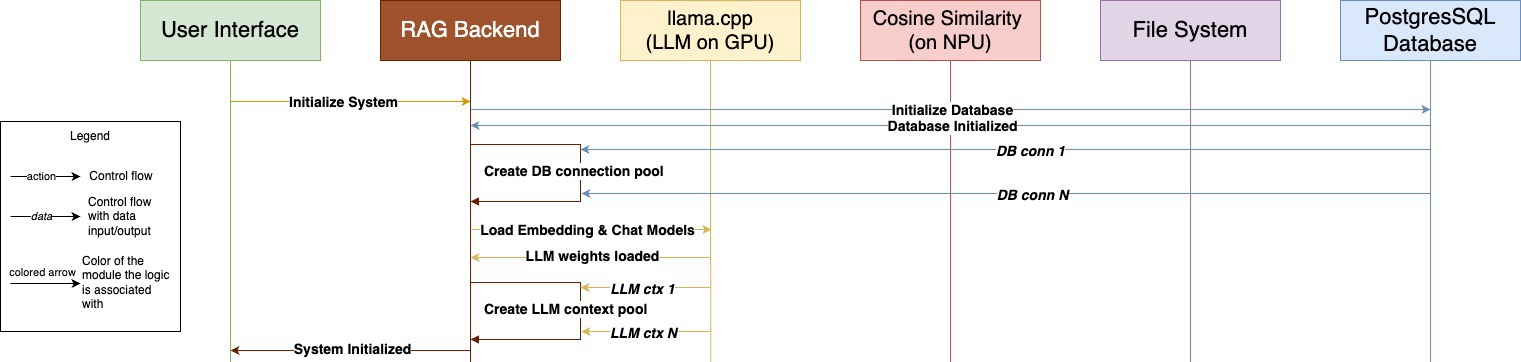
\includegraphics[width=1.0\linewidth]{images/tldr-app-worklfow-pt1.jpg}
    \caption{System initialization workflow}
    \label{fig:tldrsysteminitworkflow}
\end{figure}


The initialization phase sets up the backend infrastructure and prepares the application for use. This includes:

\begin{itemize}
    \item The user launches the application, triggering the backend.
    \item The \textbf{RAG Backend} initializes a connection pool to the \textbf{PostgreSQL Database}.
    \item The LLM weights and context pools are loaded via \texttt{llama.cpp}, enabling multi-threaded inference.
    \item Cosine similarity routines are prepared via the \textbf{NPU accelerator} module.
    \item System status is communicated back to the \textbf{User Interface}, indicating readiness.
\end{itemize}


%----------------------
\subsubsection{Embedding the Corpus}
\label{subsec:AppDesignWorkflow-EmbeddingCorpus}
%----------------------

\begin{figure}[H]
    \centering
    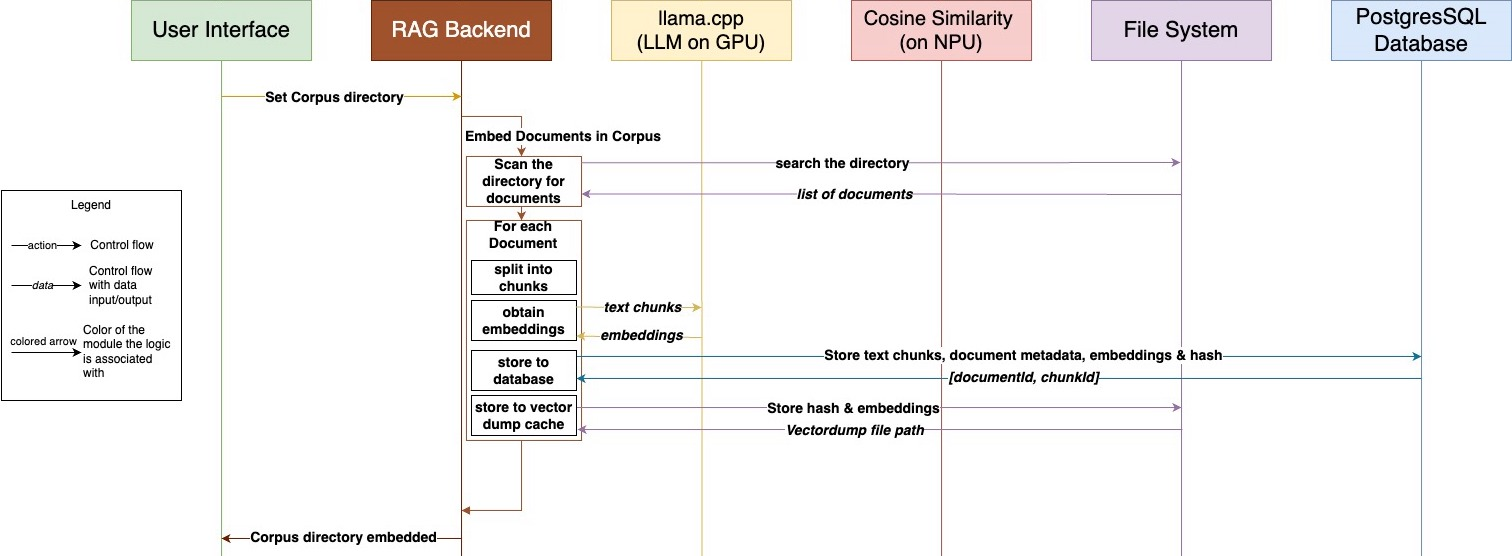
\includegraphics[width=1.0\linewidth]{images/tldr-app-worklfow-pt2.jpg}
    \caption{Corpus Embedding Workflow Steps}
    \label{fig:corpusembedworkflowsteps}
\end{figure}

When a user selects a directory to embed, the following actions take place:
\begin{itemize}
    \item The \textbf{RAG Backend} scans the specified directory for documents using the File System.
    \item Each document is loaded, chunked, and converted to embeddings using a pre-defined embedder.
    \item Embeddings, text chunks, and associated metadata are inserted into the \textbf{PostgreSQL Database}.
    \item In parallel, the backend also writes a vector dump file to the \textbf{File System}, which stores the hash of each vector for quick access.
\end{itemize}
This dual-storage mechanism (DB + mmap vector cache) allows fast retrieval during inference while maintaining queryable metadata.

%----------------------
\subsubsection{Performing RAG}
\label{subsec:AppDesignWorkflow-PerformingRAG}
%----------------------
\begin{figure}[H]
    \centering
    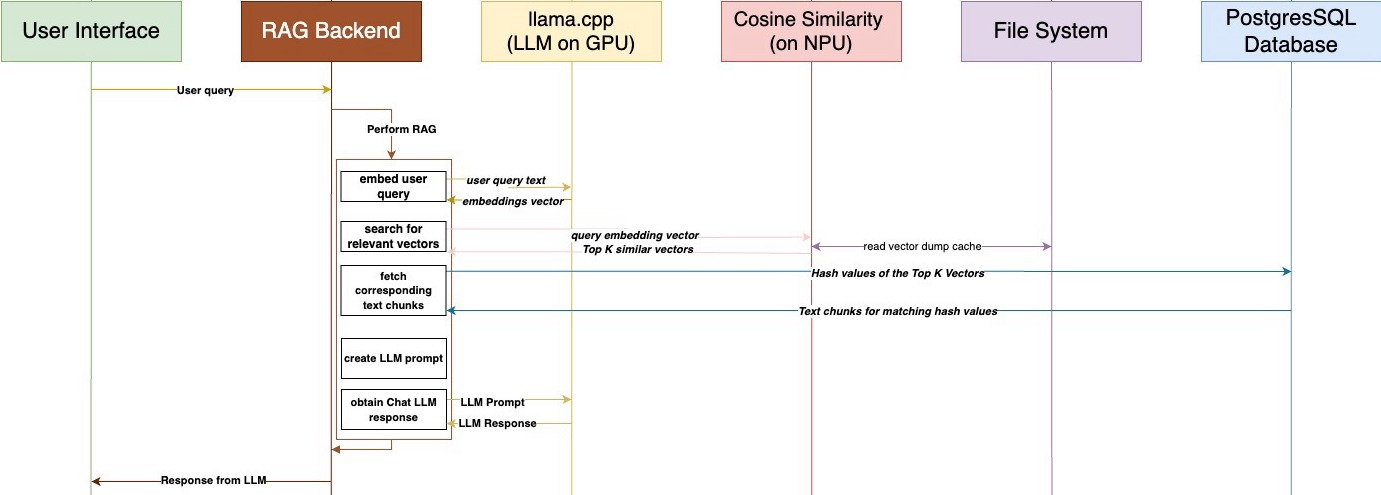
\includegraphics[width=1.0\linewidth]{images/tldr-app-worklfow-pt3.jpg}
    \caption{RAG workflow steps}
    \label{fig:ragworkflowsteps}
\end{figure}

Once the corpus is embedded, the system is ready to answer user's queries. When the user proceeds to inquire the system, the following steps are executed:

\begin{itemize}
    \item The user query is embedded using the same embedding model.
    \item The embedded query vector is sent to the \textbf{Cosine Similarity} module running on the NPU.
    \item A top-$k$ similarity search is performed against memory-mapped vector files using the NPU, returning hash values of the best matches.
    \item These hashes are used to retrieve the corresponding text chunks from the \textbf{PostgreSQL Database}.
    \item A prompt is constructed and sent to the \textbf{LLM} via \texttt{llama.cpp}.
    \item The generated response is sent back to the \textbf{User Interface}.
\end{itemize}


With these steps, the TLDR project is able to perform retrieval-augmented generation on documents present in the user's device, without requiring any external resources or internet access.


% ============================================================
%
%                   CHAPTER 5: RESULTS
%
% =============================================================

\chapter{Experimentation-TODO}
\label{ch:Experimentation}

This chapter covers the experiment design and setup, describing in detail results obtained during different phases and tests. This chapter is organized as follows: first, we discuss the results of the training and its validation in Section~\ref{sec:TrainingResults}, then in Section~\ref{sec:AutoencoderResults} and Section~\ref{sec:GeneratorResults} we explore the DL model performance from the perspective of each component individually using the methods defined in Section~\ref{sec:EvaluationMethods}.  Lastly, in Section~\ref{sec:ModelPerformance}, we analyze the performance of the DL model based on the two main evaluation metrics defined in Section~\ref{sec:ResearchObjectiveandSolution} (MSE and execution time).

Results from experiments in this chapter are based on the dataset described in Section~\ref{sec:DataCollection}. The experiments performed can be categorized into two main types based on the obstacle shape used:
\begin{enumerate}
    \item Circular obstacle: the obstacle is randomly positioned in the simulation space, and its size is given by radius $\textbf{r} = qH$, where $q \in [\frac{1}{9}, \frac{1}{5}]$ and $H$ is the height of the simulated region.
    
    \item Elliptical obstacle: the obstacle is also randomly positioned in the space, and its size is given by semi-major axis $\textbf{a}=qH$, where $q \in [\frac{1}{5}$, $\frac{1}{3}]$ and $H$ is the simulated region height, and the semi-minor axis $\textbf{b}=p\textbf{a}$, where $p \in [\frac{1}{5}, \frac{1}{4}]$. The ellipse is also tilted with an angle $\boldsymbol{\alpha} \in [-30^\circ, 30^\circ]$ with respect to $\textbf{a}$ and the Cartesian $x$-axis.
\end{enumerate}

The ranges of the obstacle dimensions and positions were chosen to fully fit the shape inside the simulated space without touching its perimeter. The dimensions of the Ellipse object were chosen to maintain a shape similar to that of an airfoil as described in Section~\ref{sec:DataCollection}, and its inclination range to represent common wing ``angle of attack" including the critical or stalling ``angle of attack" (typically between $18^\circ$ and $25^\circ$ degrees)\cite{abbott_ira_h_summary_1945}.


%----------------------
\section{Training Results}
\label{sec:TrainingResults}
%----------------------

The neural network was trained for 500 epochs, across which, the Mean Squared Error (MSE) loss functions results were collected for both the Autoencoder and the Generator. The training error is captured in  Both plots in Figure~\ref{fig:loss} show that the is generally lower than the validation error; this is to be expected given the proposed model was evaluated with sequences used during the training process. 

\begin{figure}[H]
    \centering
    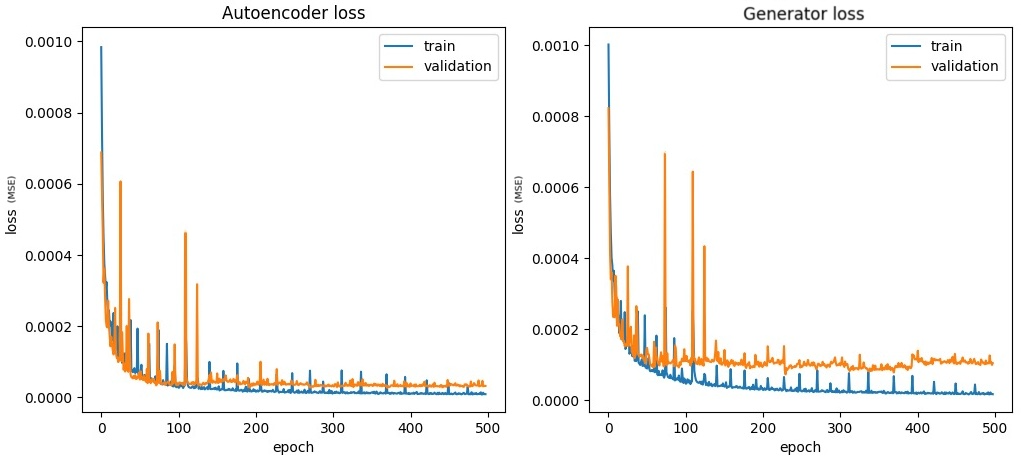
\includegraphics[width=1\linewidth]{images/model_training.png}
    \caption{Autoencoder and Generator loss evolution during training}
    \label{fig:loss}
\end{figure}

Figure \ref{fig:loss} demonstrates the stability of the MSE loss function's evolution during training. The loss trend quickly descends, and after 200 epochs, the error stabilizes and converges to its final value. In addition, note that the slight difference between the training and validation errors signifies that the model does not excessively over-fit the training data. Regular error spikes appear during training, representing instances where the model encountered local maximums before finding a local minimum. This happens when, during parameter optimization, a new combination of the network’s weights is worse than the previous one, but then it improves again. This further underscores the model's reliability. These spikes decrease as the training advances, indicating a stable and reliable training process. Another critical aspect to note is that those spikes happen almost on the same epoch number and with a similar intensity for both of the model's components (Autoencoder and Generator), meaning that these components are working in collaboration to find the best result. This supports the election of the model architecture.

\begin{table}[h]
    \caption{Training and Testing errors (MSE)}
    \centering
    \begin{tabular}{|c|c|c|}
    \hline
             & Autoencoder & Generator \\ \hline
    Training & $7.7727\times10^{-06}$ & $1.5429\times10^{-05}$ \\ \hline
    Validation  & $3.2173\times10^{-05}$ & $2.0414\times10^{-05}$ \\ \hline
    \end{tabular}
    \label{tab:errors}
\end{table}

A comparison between training and validation errors is displayed in Table~\ref{tab:errors} for both the Autoencoder and Generator components of the model. The low error rate in all cases indicates the model's good performance. It is important to remember that validation samples were not used during training, which is noticeable in how lower the training errors are compared to the validation errors. Since the model has already ``seen" the training samples to optimize its weights, it learns how to approximate the output based on those values.

In the following sections, we analyze the model's performance more deeply, examining each component's performance individually.

%----------------------
\section{Autoencoder Results}
\label{sec:AutoencoderResults}
%----------------------

To evaluate the Autoencoder, we need to verify that the Decoder can reconstruct the original information using the low-resolution representation of the data created by the Encoder. Because the input to the model is a set of frames according to the window described in Chapter~\ref{ch:Methods}, the Decoder output will also have those dimensions. This means that to evaluate the Decoder's output, we must compare all the frames in the set. 

Using the Decoder's output sequence representing the fluid state, a \textit{heatmap} of fluid velocity values was rendered to compare the results visually. Figure~\ref{fig:ReconstructedFrames} shows examples of frames with each type of obstacle. In each case, we show the Original frame to the left and the Reconstructed frame output by the Decoder to the right. We can see that although there are some minor differences, both frames are almost identical. Similar results were obtained for the rest of the sequences. The differences found can be seen in small changes of intensity of the \textit{heatmap} colors, which may indicate that the velocity values approximate the original ones but are either lower or higher than expected. Although there are some minor differences, the similarities between the Original and Reconstructed frames give us a clue that the Autoencoder is working as intended.

\begin{figure}[!htbp]
    \centering
    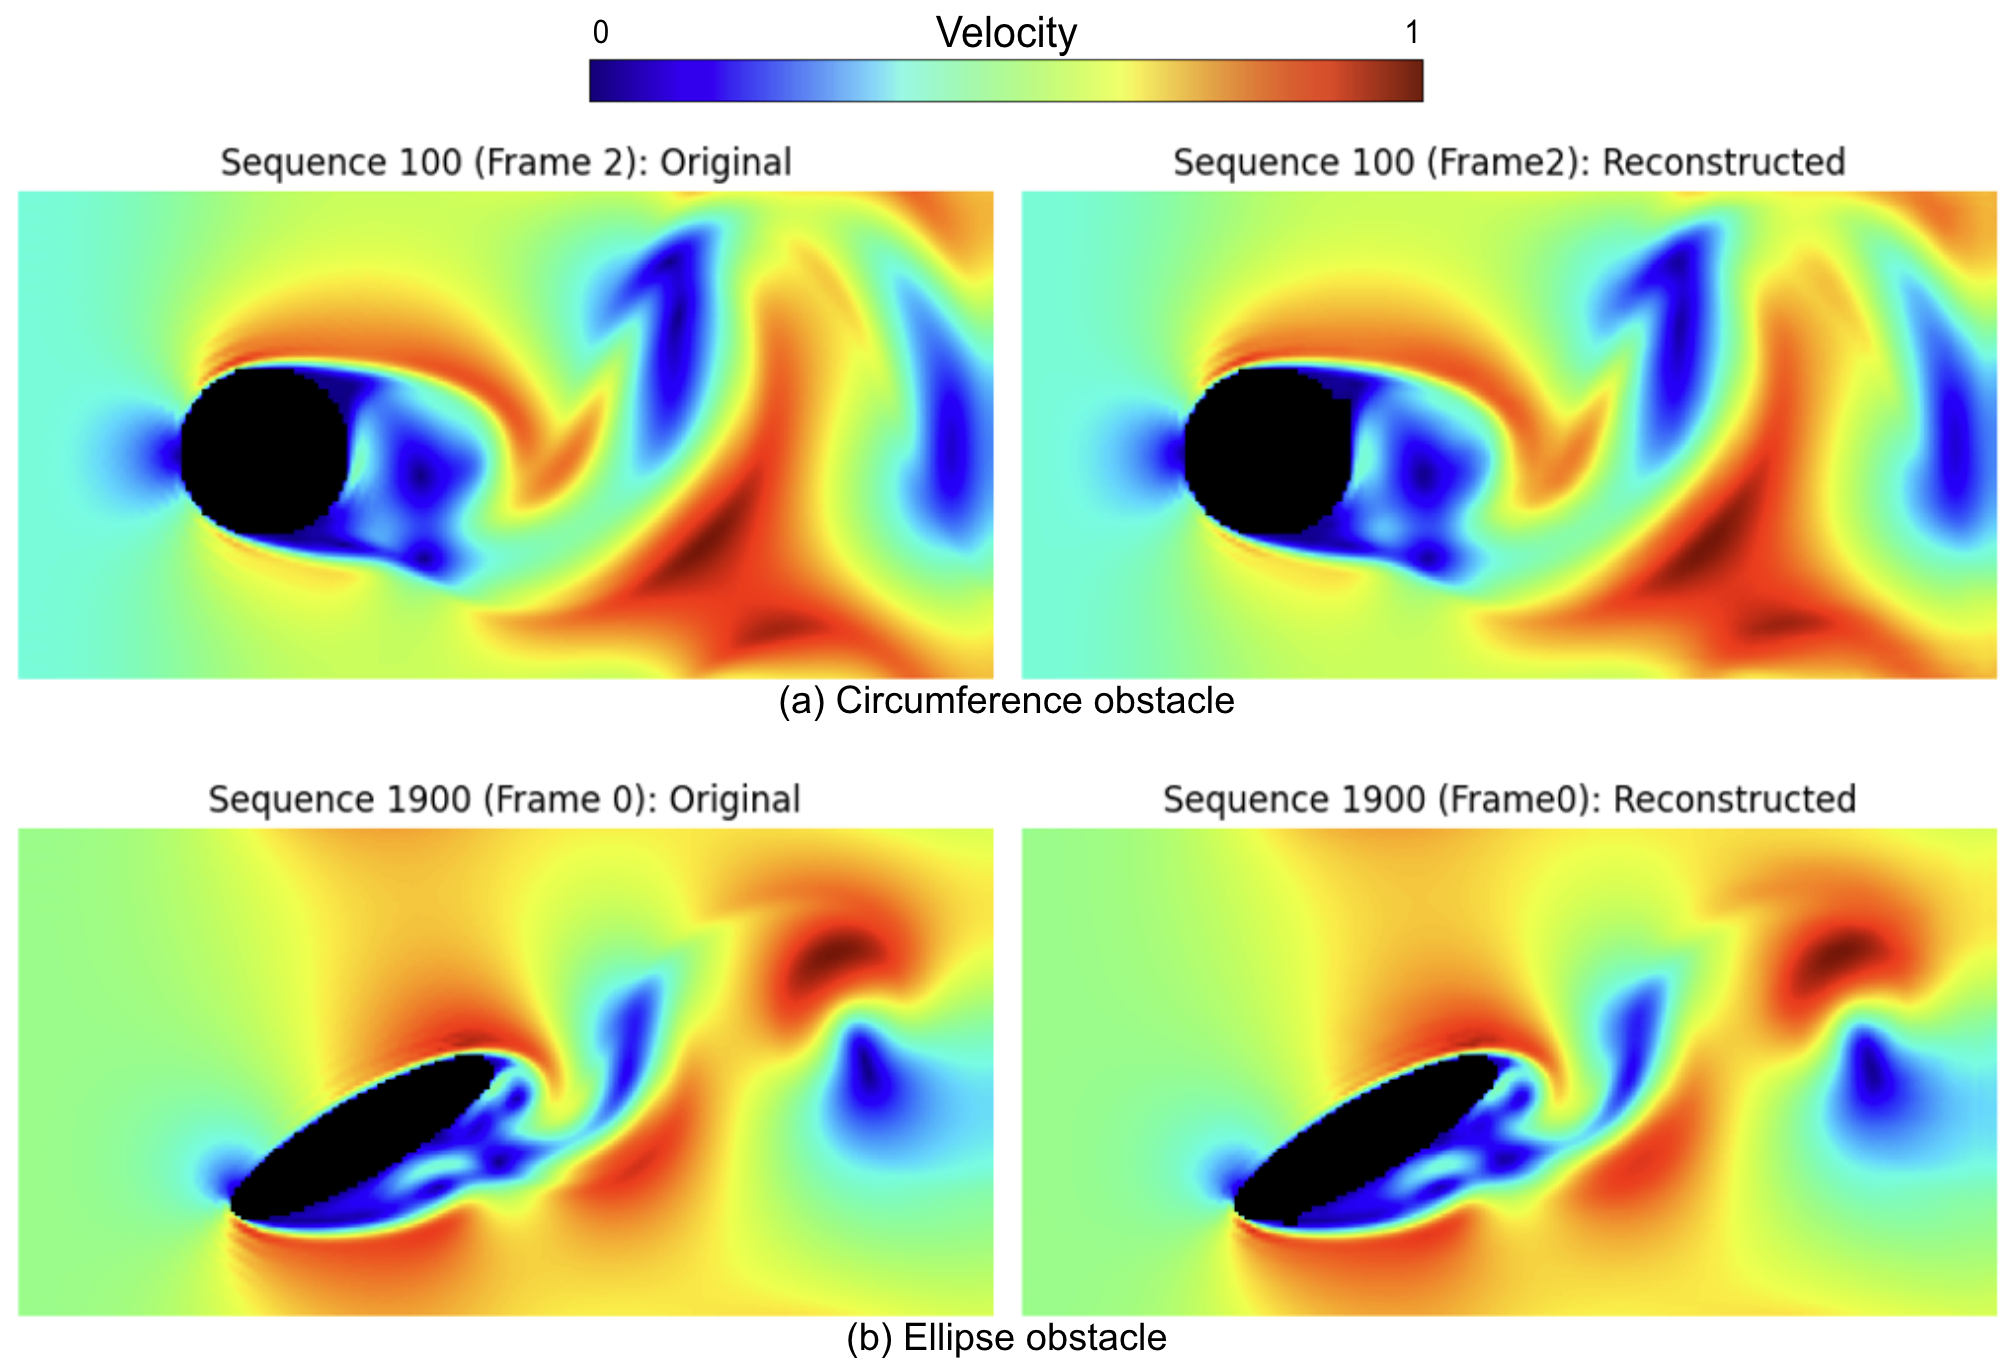
\includegraphics[width=1\linewidth]{images/autoencoder_frames.png}
    \caption{Original vs Reconstructed frames}
    \label{fig:ReconstructedFrames}
\end{figure}

For the following evaluation method, we compare the velocity values between the Original and Reconstructed frames to verify their similarity. This is done by creating a histogram of velocities, i.e., a frequency count of velocity values on each grid cell in the frame. Figure~\ref{fig:ReconstructedHistograms} shows examples of those histograms for Origianl and Reconstructed frames containing each type of obstacle. The frame examples are the same as Figure~\ref{fig:ReconstructedFrames} used in the previous evaluation method. On the x-axis, we have the range of all the velocity values in the frame. These values are between 0 and 1 because the data was previously normalized, as explained in Section~\ref{sec:DataPreparation}. On the y-axis, the frequency or occurrence of each velocity value is represented. To compare all the velocity histograms, we calculated the Jensen-Shannon distance between each frequency distribution. The resulting average distance between the original and reconstructed frames was 0.021, with a standard deviation of 0.014.

% In the example shown, we can see a lot of coincidence between the corresponding histogram bars of each frame. Similarly to the previous evaluation, we can see some differences between the histogram bars, but nothing significant. Some of the bars are taller or shorter, coinciding with the color intensity difference observed in the \textit{heatmaps} of the previous evaluation. Similar results were observed on the histograms of other sequences.

\begin{figure}[H]
    \centering
    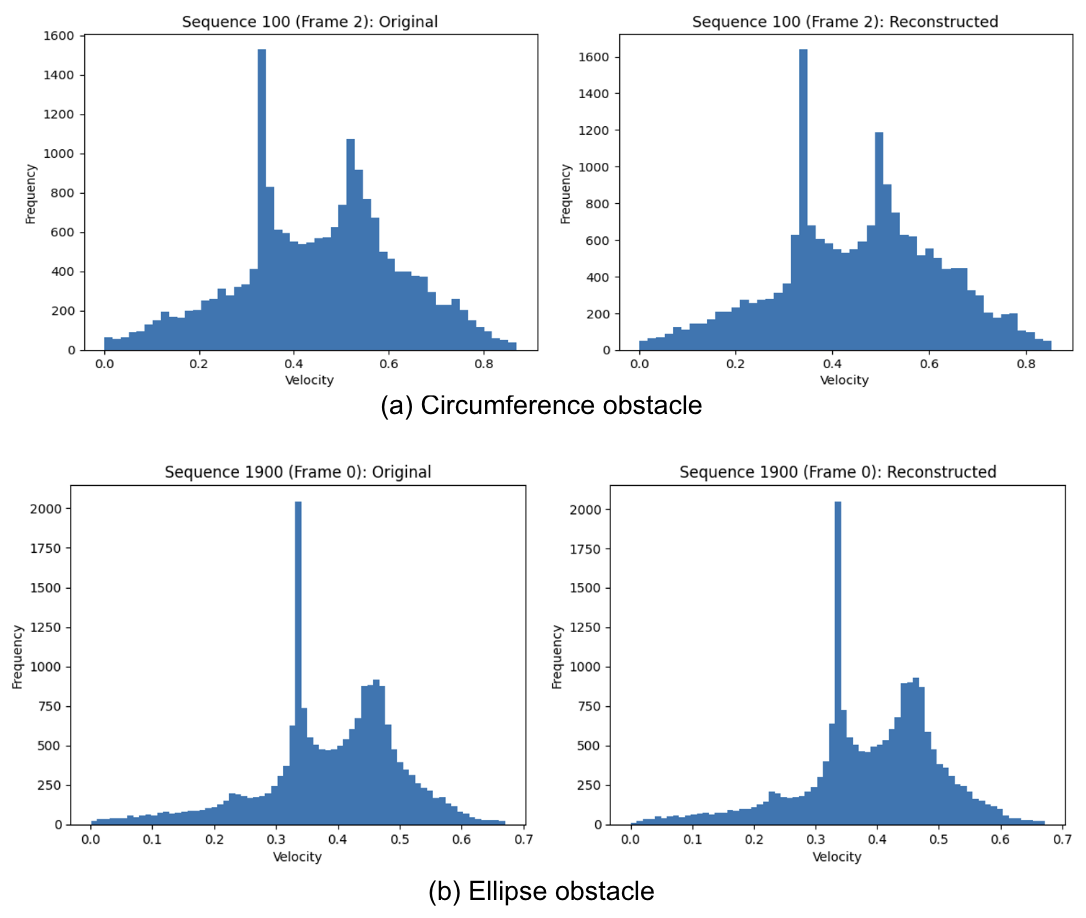
\includegraphics[width=1\linewidth]{images/autoencoder_histogram.png}
    \caption{Original vs Reconstructed frames velocity histograms}
    \label{fig:ReconstructedHistograms}
\end{figure}

Both evaluations tell us that the Autoencoder successfully reduces the data's dimensionality so that the original data can be reconstructed using that low-resolution representation. This means that the training of this model's component was successful. Although there are some minor errors, the fluid flow structure remains correct, and the approximations of the velocities are very close.

The Autoencoder is a vital component of the model because it guarantees that the model successfully extracts enough information to represent the original data. This process of reducing the amount of information with a lower representation is important to support the next phase, which is the generation of the next fluid state.

%----------------------
\section{Generator Results}
\label{sec:GeneratorResults}
%----------------------

The Generator's goal is to generate the next fluid flow state using as an input the low-resolution representation created by the Encoder. To evaluate this component, the resulting frame is compared against the expected frame taken from the dataset created by the numerical simulation. For this evaluation we used similar methods than the Autoencoder evaluation.

Figure~\ref{fig:GeneratedFrames} shows a comparison between a generated frame velocity \textit{heatmap} at the right, and the expected frame at the left. The images show a result example for each of the possible obstacle types. Similar to the Autoencoder results, very small differences appear in the \textit{heatmap} colors, however, both images are almost similar.

We created the velocity histogram for each generated frame and compared it to the original frame. Figure~\ref{fig:GeneratedHistograms} compares 2 examples of the velocity histograms. Then, we calculated the Jensen-Shannon distance between the velocity distributions of the frames in all the sequences. This results in an average distance between the expected and generated frames of 0.043 with a standard deviation of 0.010. The low average value of the distance metric between both distributions indicates that the original and generated frames are very similar.

\begin{figure}[!htbp]
    \centering
    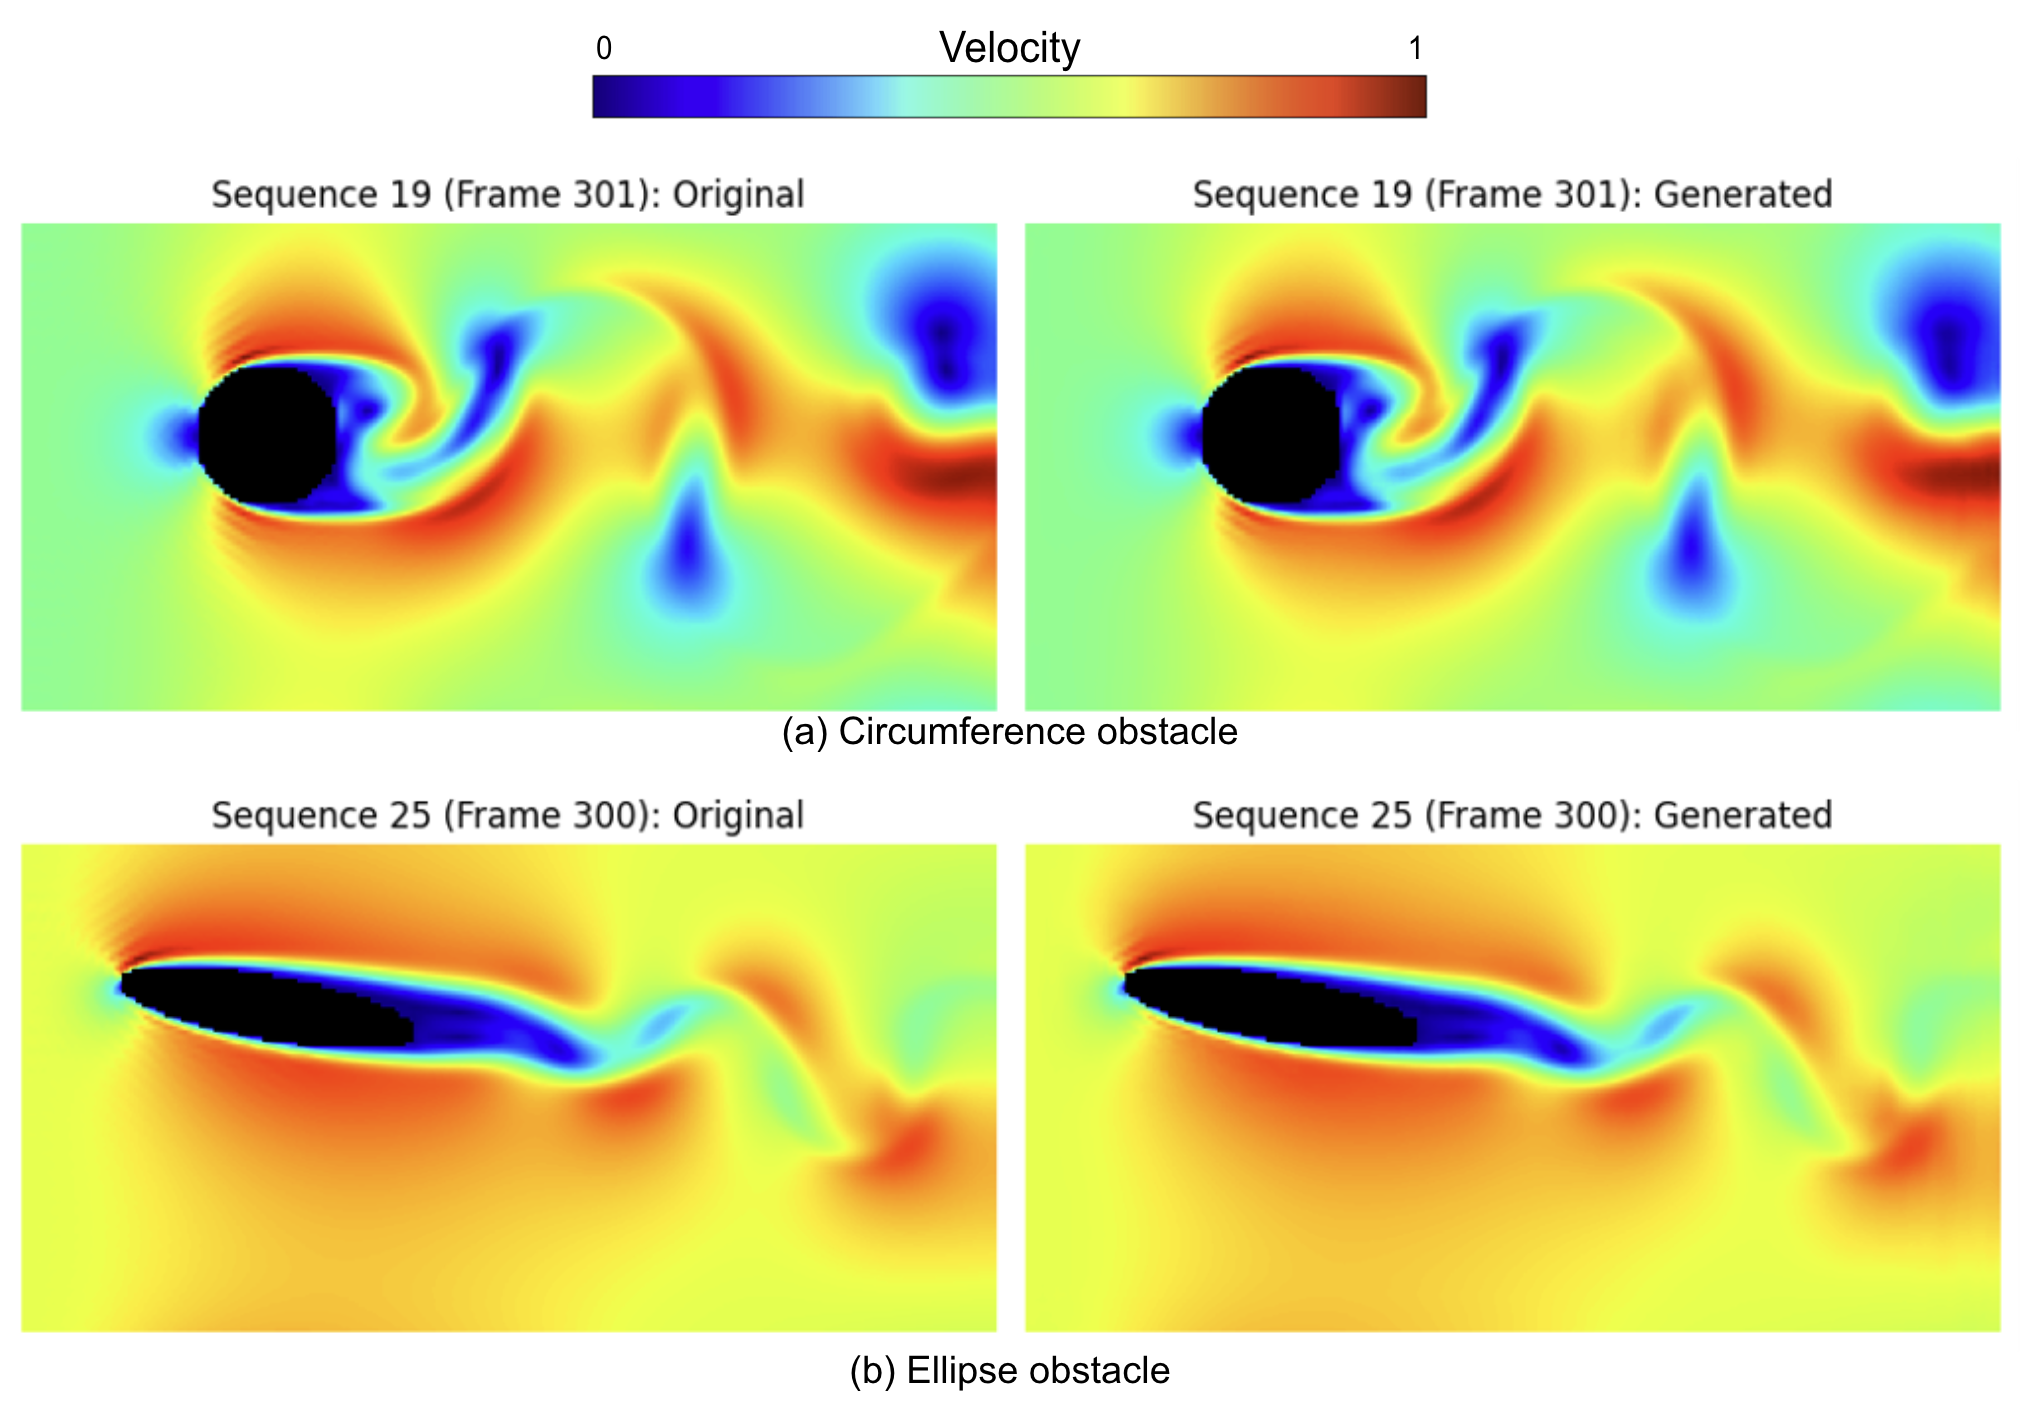
\includegraphics[width=1\linewidth]{images/generator_frames.png}
    \caption{Original vs Generated frames}
    \label{fig:GeneratedFrames}
\end{figure}

\begin{figure}[!htbp]
    \centering
    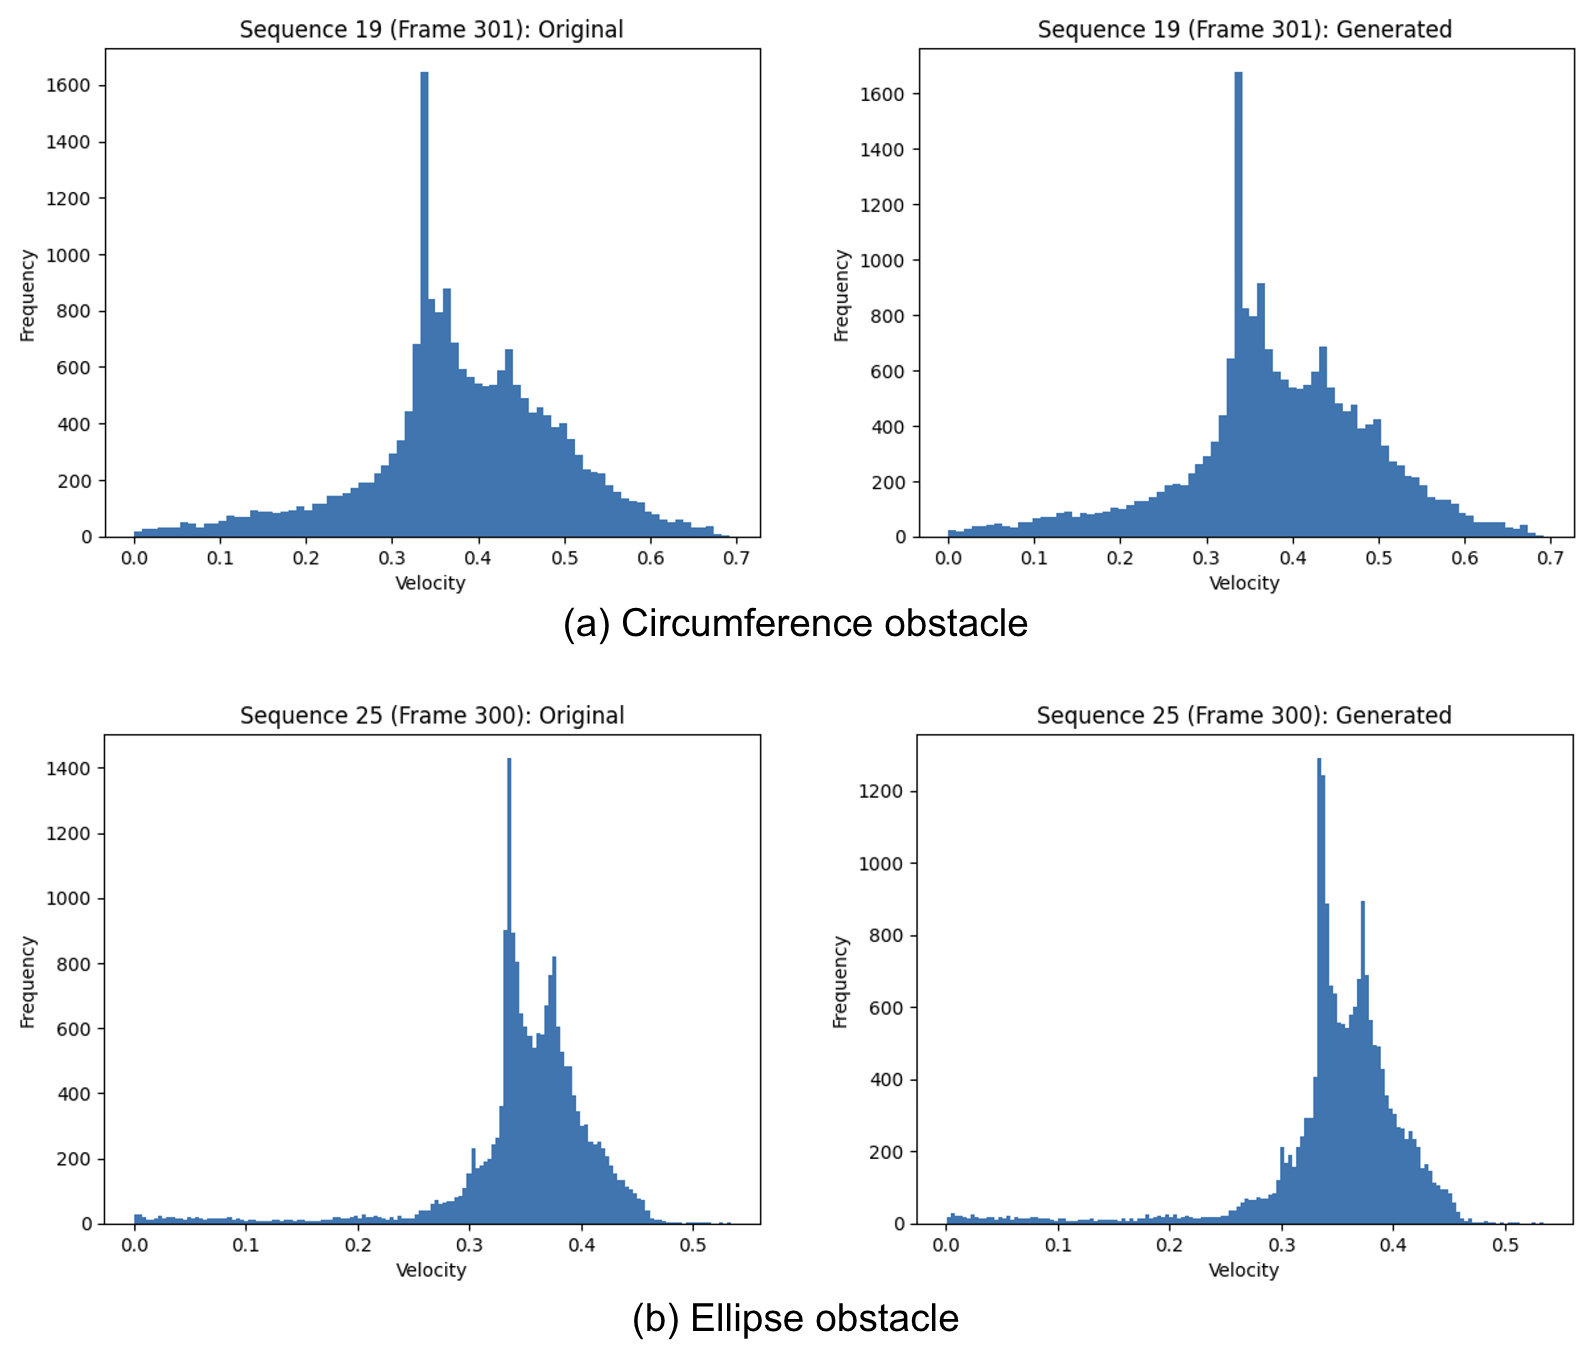
\includegraphics[width=1\linewidth]{images/generated_histogram.png}
    \caption{Original vs Generated frames velocity histograms}
    \label{fig:GeneratedHistograms}
\end{figure}


These evaluations show that the model can successfully approximate the next state in the fluid flow sequence. The same level of accuracy in both evaluation methods was observed across all the cases in the testing dataset. Although there are some differences between the expected and generated frames, the model can replicate the evolution of the fluid flow structure across the sequence simulation time.

%----------------------
\section{Model Performance}
\label{sec:ModelPerformance}
%----------------------

In this section we explore the results of the two main metrics chosen to evaluate this models performance as explained in Section~\ref{sec:ResearchObjectiveandSolution}. These metrics are: the Error measured with MSE, and the execution time of the simulation measured in seconds.

\subsection{Error Measurements}
\label{subsec:ErrorMeasurements}

Figure~\ref{fig:ErrorMeasurements} shows the results of the MSE metric. The results are divided into three groups, one for all the shapes in the dataset together, one with only Circumferences obstacles, and another for Ellipses obstacles. The minimum, maximum, and average error values are plotted for each group. It is important to mention that the dataset is balanced, meaning that the amount of examples with each obstacle type is the same, which is essential to ensure fairness in the results. 

The following analysis can be done by looking at the MSE plots in Figure~\ref{fig:ErrorMeasurements}. We can see that the minimum and maximum errors across the entire dataset are both in simulations with an ellipse obstacle. Additionally, the difference between the minimum and maximum error is lower for the circumference than the ellipse obstacle. This could be caused by circumference obstacles presenting less variability in their shapes, with only a change in the radius, while ellipses obstacles have more diversity in their shapes. This variability in the obstacle shapes makes it more challenging for the model to learn how to simulate the ellipse objects. However, because the average errors are similar between the two types of obstacles, we can conclude that no specific obstacle shape is significantly more difficult for the model to simulate. 

\begin{figure}[!htbp]
    \centering
    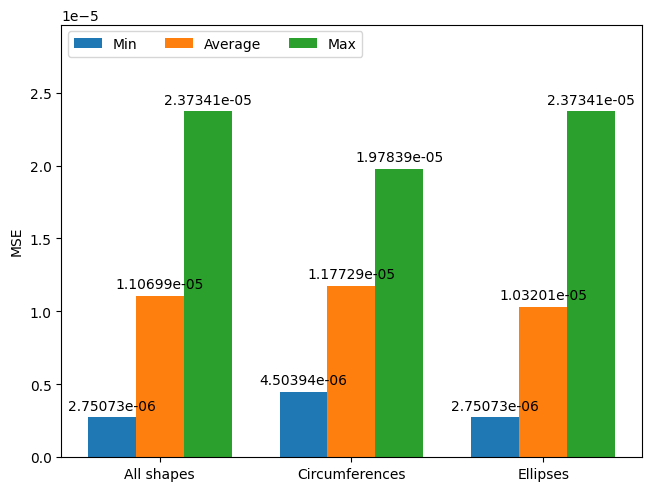
\includegraphics[width=0.7\linewidth]{images/MSE.png}
    \caption{Model MSE error metric}
    \label{fig:ErrorMeasurements}
\end{figure}


\subsection{Execution time}
\label{subsec:ExecutionTime}
As explained in Section~\ref{sec:ResearchObjectiveandSolution}, the goal of this model is to reduce the execution time of the simulation while maintaining a low error to preserve the pattern structure of the fluid flow in the generated sequence. Table~ \ref{tab:ExecutionTime} compares execution time between the simulation and the DL Model. The simulation took, on average, 191 seconds (3.2 minutes), while the DL model took, on average, only 42 seconds. This represents a 4.5 times improvement in execution speed over the numerical simulation. This result shows that using this DL model improves the simulation's performance, reducing the total execution time while successfully simulating the evolution of the fluid flow. 


% \begin{figure}[!htbp]
%     \centering
%     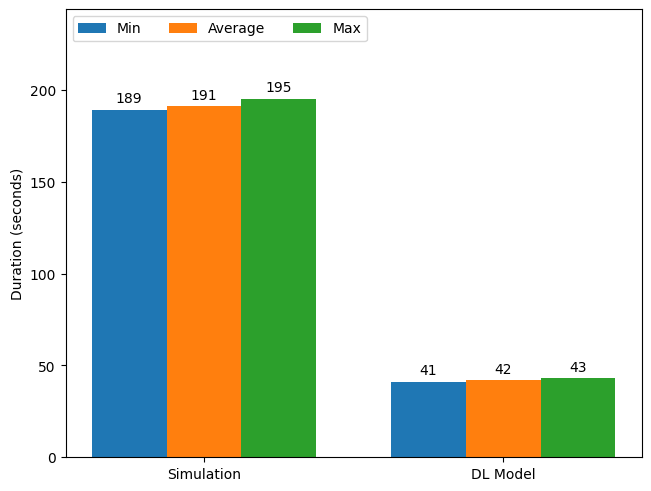
\includegraphics[width=0.7\linewidth]{images/execution_time.png}
%     \caption{Model execution time}
%     \label{fig:ExecutionTime}
% \end{figure}


\begin{table}[ht]
    \caption{CFD simulation vs DL Model execution time}
    \centering
    \begin{tabular}{|c|c|}
    \hline
                    & Average Execution Time \\ \hline
    CFD Simulation  & 191 \\ \hline
    DL Model        & 42 \\ \hline
    \end{tabular}
    \label{tab:ExecutionTime}
\end{table}



% ============================================================
%
%                   CHAPTER 6: CONCLUSION
%
% =============================================================

\chapter{Conclusion}
\label{ch:Conclusion}

% % --------------------------------------
\section{Takeaways}
\label{sec:Takeaways}
% % --------------------------------------
The following are the key takeaways of this project:
\begin{enumerate}[label=\alph*.]
\item Apple Neural Engine (ANE) Utilization: This project explored leveraging the underused NPU for LLM inference, going beyond standard CoreML use cases and showed that it can be viable.

\item Retrieval-Augmented Generation (RAG) without Internet : Implements a lightweight RAG pipeline that only uses on device resources.

\item Portability and Ease of use: Application size of less than 1GB that includes everything, available for download at \href{https://tldr.cool}{\textbf{https://tldr.cool}}

\item Quantized LLMs: Uses compact models (50–500MB) for efficient, on-device inference allowing for seamless multitasking and manages to obtain results comparable to mainstream cloud LLMs.
\end{enumerate}
% % --------------------------------------
\section{Limitations}
\label{sec:Limitations}
% % --------------------------------------
Following are the main limitations uncovered during the implementation of this project:
\begin{enumerate}[label=\alph*.]
\item While this project demonstrates the feasibility to accelerate the retrieval part of the RAG pipeline, the LLM Inference still only leverages the GPU and does not leverage the NPU.

\item Indexing(embedding) takes 90+% of overall runtime

\item Many smaller LLMs available currently (3B or less) are only instruction-tuned i.e trained for text completion and not for chat. This can lead to unfavorable responses during chat.

\item Excessive usage limits to quick draining of power, especially on portable devices.

\item The breadth of retrieval space is limited not by resources but by the context size of the Chat LLM, since both input and expected output must fit in the LLM context.

\end{enumerate}
% % --------------------------------------
\section{Future work}
\label{sec:FutureWork}
% % --------------------------------------
\begin{enumerate}[label=\alph*.]
    \item Enhance data safety mechanisms for vectordump files.
    \item Add NPU backend for GGML and llama.cpp.
    \item Quantize and convert fine-tuned chat-optimized LLMs to the GGUF format.
    \item Implement a dedicated parallelized tokenization module.
    \item Extend the application support beyond Apple Silicon.
    \item Add NPU and GPU acceleration support for SQLite and Postgres vector search extensions (they currently only support CPU).
    \item Create an optimized decoding and tokenization workflow dedicated for embedding (e.g., no KV cache).
\end{enumerate}

\printendnotes

%
% ==========   Bibliography
%
% \nocite{*}   % include everything in the uwthesis.bib file
\bibliographystyle{unsrt}
\bibliography{uwthesis}
%
% ==========   Appendices
%

\end{document}